\chapter{Neuron Parameter Evaluation and Optimisation}
\label{chp:neuron_evaluation}

\glsunset{LIF}
\glsunset{AdEx}

A primary goal of this thesis is to explore the design space of the spiking \acrshort{BiNAM} implementation presented in \cref{chp:spinam}. In this chapter we summarise and categorise the design space parameters introduced in the preceding two chapters and discuss two strategies for design space exploration: full network and single neuron evaluation. Whereas the first strategy evaluates entire \acrshort{BiNAM} networks according to memory performance measures, this chapter focuses on the second strategy, which examines how well a single neuron with parameters \nParams matches the threshold and reset conditions introduced in \cref{sec:required_neuron_behaviour}.

\cref{sec:design_space} elaborates on single neuron and full network evaluations, and motivates single neuron evaluation as an approximation of full network evaluation. \cref{sec:single_neuron_simulation} details the implementation of the single neuron simulator, which is a building block of the individual evaluation measures discussed in \cref{sec:spike_train_measure,sec:sgso_measure,sec:sgmo_measure}. A glimpse at the corresponding software toolchain is given in \cref{sec:adexpsim}. This toolchain is then used to compare the measures regarding their accuracy and suitability for automated parameter optimisation in \cref{sec:single_neuron_measure_comparison}.

\section{Design space exploration}
\label{sec:design_space}

This section compares two complementary strategies to design space exploration: full network exploration on the one hand, introduced in \cref{chp:spinam}, and single neuron evaluation on the other hand, the primary topic of this chapter. Before we set out to discuss design space exploration, we need to clarify the notions of \enquote{design space} and \enquote{exploration}. The first part of this section summarises the design space parameters described in \cref{chp:related_work,chp:spinam}, while the second and third part elaborate on the already mentioned exploration strategies. The fourth and final part discusses to what extent the design space dimensionality can be reduced and which constraints have to be imposed on the parameter combinations.

\subsection{On the terms \enquote{design space} and \enquote{exploration}}
\label{sec:design_space_defn}

\begin{table}
	\centering
	\small
	\renewcommand{\arraystretch}{1.4}
	\begin{tabular}{p{3.5cm} p{3.5cm} p{3.5cm}}
		\toprule
		\multicolumn{3}{c}{\spacedlowsmallcaps{Design space overview}} \\

		\midrule
		\multicolumn{3}{c}{\textit{System parameters}} \\
		\midrule
		\spacedlowsmallcaps{Network} & \spacedlowsmallcaps{Encoding} & \spacedlowsmallcaps{Noise} \\
		Memory size \dimIn, \dimOut & Burst size \burstSizeIn, \burstSizeOut & False pos./neg. \pFp, \pFn \\
		Number of \enquote{ones} \nOnesIn, \nOnesOut & Interspike interval \isi & Time noise \jitter, \jitterOffs\\
		Sample count \nSamples & Sample interval \timeWindow & Neuronal noise \jitterNParam$\Box$ \\
		Population size \populationSize & & \\
		\midrule
		\multicolumn{3}{c}{\textit{Neuron parameters}} \\
		\midrule
		\spacedlowsmallcaps{Synapse} & \spacedlowsmallcaps{Membrane (LIF)} & \spacedlowsmallcaps{AdEx} \\
		Weight \wsyn & Capacitance \Cm$\circ$ & Adaptation \Ga, \ib \\
		Rev. potentials \Ee, \Ei$\diamond$ & Leak potential \El$\circ$ & Time constant \TauA \\
		Time constants \TauE, \TauI$\diamond$ & Threshold \ETh$\circ$ & Exp. threshold \EThExp \\
		& Leak conductance \Gl & Exp. slope \DT \\
		& Reset potential \Ereset \\
		& Refractory period \TauRef \\
		\bottomrule
	\end{tabular}
	\caption[Overview of variables in the design space]{Overview of variables in the design space. $\diamond$ Inhibitory synapses are not used in the \BiNAM network, so the parameters \Ei and \TauI can be ignored. $\circ$ Superfluous degrees of freedom (\cref{sec:parameter_normalisation}). $\Box$ There is an individual noise parameter for each neuron parameter $\phi$.}
	\label{tbl:design_space}
\end{table}

\marginnote{Detailed information on the system parameters can be found in the previous chapter \ref{chp:spinam}, both the \acrshort{LIF} and \acrshort{AdEx} model and their parameters are presented in \cref{sec:spiking_neuron_models}.}
The \BiNAM design space can be partitioned into two disjunct sets of parameters: \emph{system} and \emph{neuron} parameters. System parameters specify the spike time encoding of input and output data, the amount of noise present on the platform, and the memory size and data characteristics. The neuron parameters \nParams control the behaviour of the dynamical systems which constitute the network. Number and availability of neuron parameters depends on the chosen model. Here, we either chose the \acrfull{LIF} model or its extension, the \acrfull{AdEx} model. From a practical point of view, the most important distinction between neuron and system parameters is that system parameters are constant, external parameters, whereas the neuron parameters \nParams must be tuned with respect to the system parameters, such that they fulfil the task specified by the memory parameters and encoding scheme, while constrained by the noise in their environment. \cref{tbl:design_space} summarises the $16$ neuron and $30$ system parameters ($14$ plus $16$ for neuronal noise).

At this point, we must distinguish two major applications of design space exploration. Sweeping over a static, manually defined subspace of the design space allows to compare the behaviour of the \BiNAM on different platforms, which is potentially useful as a platform benchmark. The second application of design space exploration is parameter optimisation. Here, we try to find parameters, which optimise the memory with respect to one or multiple evaluation measures like those presented in \cref{sec:memory_evaluation_measures}. The optimisation process can be either  manual, in which case an interactive visualisation of the design space is beneficial, or automated, in which case \enquote{smooth} gradients in the evaluation measures are favourable. Automated parameter optimisation facilitates the adaptation of a \BiNAM implementation to new simulator platforms and topology parameters. In the remainder of this section we focus on optimisation of a neuron parameter vector \nParams with respect to constant system parameters. Optimisation of spiking neuron parameters is a problem commonly considered as hard to solve \cite{prinz2007neuronal}.

\subsection{Full network evaluation}

\marginnote{At the time of writing, setup and postprocessing times are in the order of seconds to minutes for considerably large networks simulated on the \NMPM and \NMMC hardware systems.}
Full network evaluation is the empirical approach to design space exploration. For each distinct parameter vector a network simulation is executed and the evaluation measures presented in \cref{sec:memory_evaluation_measures} are calculated: storage capacity, latency, robustness and energy consumption. To visualise a two-dimensional sub-region of the parameter space, a network simulation can be executed for each point in a pre-defined two-dimensional grid. However, a major drawback if this methodology is the time required for network simulations. State-of-the-art neuromorphic hardware or fewer calculation points can not sufficiently alleviate this problem, because high setup and post-processing costs still apply. Naively sweeping over parameter space dimensions is off the table, as it is furthermore likely to waste vast portions of time in \enquote{uninteresting} parameter space regions, in which the neurons do not fulfil the threshold- and reset conditions required for an associative memory.

\marginfig{Membrane potential over time for a neuron with degenerate parameters causing low latency}{
	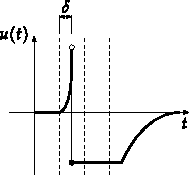
\includegraphics{media/chp4/degenerate_low_latency.pdf}
}{Sketch of $\um(t)$ for a neuron with degenerate parameters. Issuing a single output spike immediately following the first input spike (dashed) and then staying in the refractory state minimises the latency \latency.}
{\label{fig:degenerate_low_latency}}
Calculating evaluation measures in such regions of the design space would lead to trivial results. Of course, a neuron which fires a single output spike whenever it receives an input spike -- sketched in \cref{fig:degenerate_low_latency} -- would minimise the latency measure, but is useless in an actual associative memory. Classically, such degenerate solutions in multi-objective optimisation problems can be avoided by the introduction of a compound goal function which combines the aforementioned evaluation measures into a scalar optimality measure. Another means is Pareto optimisation, where parameter vector sets are searched, for which the variation of a single parameter dimension would degrade at least one of the performance measures. However, Pareto optimisation is less feasible for high-dimensional parameter spaces \cite{miettinen2012nonlinear}.

\subsection{Single neuron evaluation}
\label{sec:single_neuron_evaluation}

\begin{figure}
	\centering
	\subbottom[Individual inputs]{%
		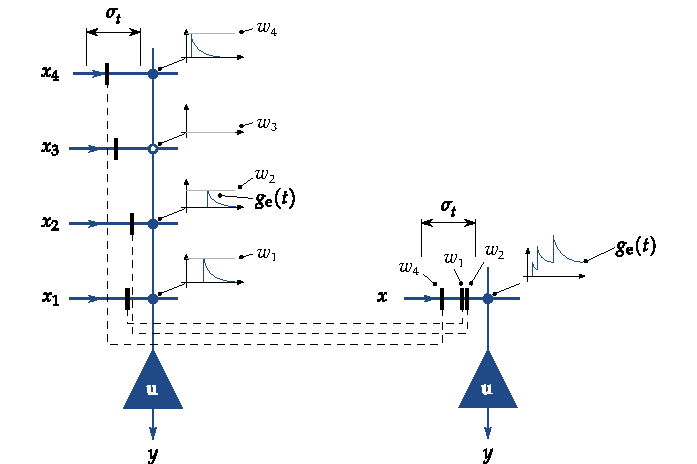
\includegraphics[trim=0.5cm 0cm 5.65cm 0cm,clip]{media/chp4/binam_timing.pdf}%
	}%
	\subbottom[Fused input]{%
		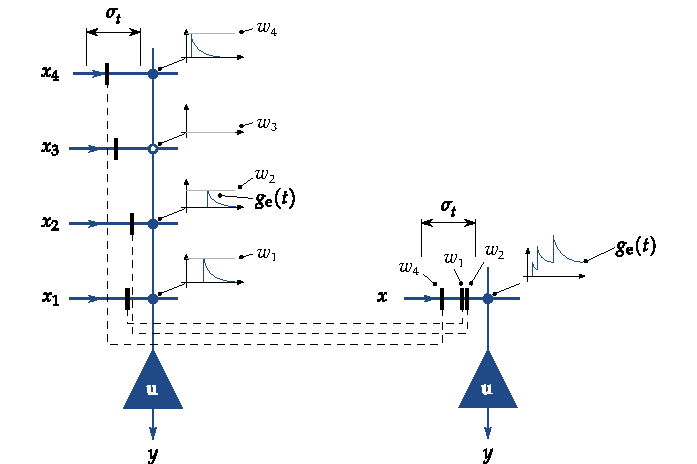
\includegraphics[trim=6.15cm 0cm 0.5cm 0cm,clip]{media/chp4/binam_timing.pdf}%
	}%
	\caption[Sketch of the input spike train fusion model]{Sketch of the input spike train fusion model. (a) shows a single neuron receiving input spikes with timings drawn from a Gaussian distribution with standard deviation \jitter. The small diagrams depict the individual synapse conductivity over time. (b) shows an equivalent setup with a single input: the input spike trains arriving at non-zero weight synapses are fused into a single spike train with annotated weights.}
	\label{fig:fusion_model}
\end{figure}

The single neuron evaluation technique evades the perils of multi-objective optimisation and focuses solely on compound measures which quantify the \enquote{optimality} of neuron parameters. This approach is possible, as the \BiNAM itself, and the spiking \BiNAM implementation presented in \cref{chp:spinam} in particular, are highly homogeneous. Each individual neuron in the network is independently responsible for a single output component $(\vOut)_i$, or, in case of neuron populations, a single signal in the output bundle. To provide an operational memory with a storage capacity close to the theoretical optimum, each neuron in the network must equally adhere to the reset and threshold conditions postulated in \cref{sec:required_neuron_behaviour}. Regarding the neuron model, an input spike arriving at a synapse just increases the excitatory channel conductance $\Ge(t)$ of the post-synaptic neuron by the synaptic weight $w_i$. The input spikes can be fused into an equivalent compound spike train, as long as they are annotated with the corresponding synaptic weight (\cref{fig:fusion_model}).

\marginnote{In the \BiNAM implementation, all synapses share the same weight \wsyn. However, we do not need to restrict our model that far, as handling of different synapse weights also allows the handling of synaptic weight noise $\sigma_{\wsyn}$.}
To summarise, given equal input, neurons in the network are supposed to exhibit the same behaviour, and the input itself can be represented by a single spike train \tIn with annotated synaptic weights \wIn. Correspondingly, design space exploration is possible by simulating a proxy neuron with parameters \nParams, one excitatory synapse with adaptive weight and an according input spike train $(\tIn, \wIn)$ which tests the neuron properties. Since the network solely consists of non-interacting copies of the proxy, its behavioural properties can be extrapolated to the entire network. In case the network is simulated deterministically by software, this reductionistic approach should accurately predict the behaviour of the network, allowing time-efficient and interactive design space exploration due to the vastly reduced complexity $\mathcal{O}(1)$ of single neuron simulation compared to the simulation of a full network in $\mathcal{O}(\dimOut)$.

However, by definition, the single neuron approach cannot account for imprecisions on neuromorphic hardware. Apart from noise that might be introduced by analogue hardware on neuron parameters and synapse weights, both analogue and digital systems can produce non-uniform spike-time latencies and loose entire spike events due to limited network capacity. This kind of noise is likely to manifest when the data parameters \dimIn, \dimOut, \nOnesIn and \nOnesOut are increased. It is improbable that the simple Gaussian noise model presented in \cref{sec:input_data_parametrisation} correctly captures this behaviour. On an even more fundamental level, it is unclear whether the hardware system -- apart from noise -- realises a given parameter combination correctly. Thus, single neuron simulation can in principle not replace the execution of full networks on neuromorphic hardware. However, it allows to identify regions in the parameter space in which neurons potentially fulfil the requirements for neurons in an operational \BiNAM spiking associative memory. Subsequently, a full network evaluation can be performed in these restricted regions.

\subsection{Parameter constraints and intra-dependencies}
\label{sec:parameter_normalisation}

With 16 dimensions, our parameter space does not lend itself to exhaustive exploration. However, by exploiting dependencies between parameters, constraints and redundancies, a smaller subspace of feasible parameters can be identified.

\paragraph{Invalid parameter combinations}
The first category of constraints in the \AdEx model parameter space stems from the natural value range of some parameters. It should be obvious, that all time constants, capacitances and conductances must be larger than or equal zero. It must hold
\begin{align}
	\Cm > 0, \Gl > 0, \TauE > 0, \TauI > 0, \TauA > 0, \TauRef \geq 0, \wsyn \geq 0, \Ga \geq 0 \,.
\end{align}
The second category contains more debatable constraints. Perhaps the model might still produce sensible results if these constraints are violated, yet assumptions made in the following sections are no longer valid. The first set of constraints imposes an order on the potential parameters. For the \AdEx model it should hold
\begin{align}
	\ETh > \Ee > \EThExp > \El \geq \Ei \geq \Ereset \,,
\end{align}
for the \LIF model, which does not possess the \EThExp parameter, it should hold instead
\begin{align}
	\Ee > \ETh > \El \geq \Ei \geq \Ereset \,.
\end{align}
The exponential slope \DT and the adaptation current \ib are subject to the constraints
\begin{align}
	\DT < \EThExp - \El, \ib \geq 0 \,.
\end{align}
Violation of the first condition may result in unstable neuron behaviour; see \cref{sec:effective_threshold_potential} for a derivation of the condition. Similarly, negative adaptation currents $\ib < 0$ excite the neuron and can trigger a self-amplifying cascade of output spikes.


\paragraph{Hardware constraints}

\begin{table}
	\small
	\centering
	\renewcommand{\arraystretch}{1.3}
	\begin{tabular}{r l r l}
		\toprule
		\multicolumn{4}{c}{\spacedlowsmallcaps{Nominal NM-PM1 AdEx parameter restrictions}} \\
		\midrule

		\textit{Parameter} & \textit{Range} & \textit{Parameter} & \textit{Range} \\
		\cmidrule(r){1-2}\cmidrule(l){3-4}

		\Cm & \SI{1}{\nano\farad} & \El & \SIrange{-125}{45}{\milli\volt}\\
		\Gl & \SIrange{1.9}{22.2}{\nano\siemens} & \Ee & \SIrange{-125}{45}{\milli\volt}\\
		\TauE & \SIrange{1}{100}{\milli\second} & \Ei & \SIrange{-125}{45}{\milli\volt}\\
		\TauI & \SIrange{1}{100}{\milli\second} & \ETh & \SIrange{-125}{45}{\milli\volt}\\
		\TauA & \SIrange{20}{780}{\milli\second} & \Espike & \SIrange{-125}{45}{\milli\volt} \\
		\TauRef & \SIrange{0.16}{10}{\milli\second} & \Ereset & \SIrange{-125}{45}{\milli\volt}\\
		\Ga & \SIrange{0}{10}{\nano\siemens} & \DT & \SIrange{0.4}{3}{\milli\volt}\\
		\ib & \SIrange{0}{86}{\pico\ampere} & \wsyn & \SIrange{0}{0.3}{\micro\siemens} (4 bit) \\
		\bottomrule
	\end{tabular}
	\caption[Nominal parameter constraints of the NM-PM1 platform]{Nominal \AdEx parameter constraints of the \NMPM platform \cite{petrovici2014characterization}. Only valid for a speedup of $10\,000$ and the specified $\Cm$.}
	\label{tbl:hw_limitations}
\end{table}

\marginnote{The parameter space of numerical simulators is limited by floating point precision, or, in the case of \NMMC the precision of the 16-bit integers in which the parameters are stored.}
Numerical spiking network simulators offer an almost unlimited parameter space. This is not true for analogue neuromorphic hardware systems such as Spikey and \NMPM, where the parameters are limited by physical constraints. Unfortunately, as the mapping from model to hardware parameters is subject to calibration, selected membrane capacitance and speedup factor, the exact limitations vary. \cref{tbl:hw_limitations} shows the nominal parameter ranges for \NMPM at the speedup of $10\,000$ and a model membrane capacitance of $\SI{1}{\nano\farad}$.


\paragraph{Superfluous degrees of freedom}

\begin{table}[p]
	\small
	\centering
	\begin{tabular}{r l l l}
		\toprule
		\multicolumn{4}{c}{\spacedlowsmallcaps{Reduced DoF AdEx and LIF parameters and neuron state}} \\

		\midrule
		\multicolumn{4}{c}{\textit{Potentials}} \\
		\midrule

		& \spacedlowsmallcaps{Unit} & \spacedlowsmallcaps{Description} & \spacedlowsmallcaps{Transformation} \\

		\noalign{\vskip 2mm}
		$\ETh'$ & $[\si{\volt}]$ & Threshold potential & $\ETh - \El$ \\

		\noalign{\vskip 2mm}
		$\EThExp'$ & $[\si{\volt}]$ & Spike potential & $\EThExp - \El$ \\

		\noalign{\vskip 2mm}
		$\Ereset'$ & $[\si{\volt}]$ & Reset potential & $\Ereset - \El$ \\

		\noalign{\vskip 2mm}
		$\Ee'$ & $[\si{\volt}]$ & Excitatory reversal potential & $\Ee - \El$ \\

		\noalign{\vskip 2mm}
		$\Ei'$ & $[\si{\volt}]$ & Inhibitory reversal potential & $\Ei - \El$ \\

		\midrule
		\multicolumn{4}{c}{\textit{Decay rates}} \\
		\midrule

		& \spacedlowsmallcaps{Unit} & \spacedlowsmallcaps{Description} & \spacedlowsmallcaps{Transformation} \\

		\noalign{\vskip 2mm}
		\Fl & $[\si{\per\second}]$ & Membrane leak rate & $\Gl / \Cm$\\

		\noalign{\vskip 2mm}
		\La & $[\si{\per\second}]$ & Adaptation decay rate & $1 / \TauA$ \\

		\noalign{\vskip 2mm}
		\Le & $[\si{\per\second}]$ & Excitatory channel decay rate & $1 / \TauE$ \\

		\noalign{\vskip 2mm}
		\Li & $[\si{\per\second}]$ & Inhibitory channel decay rate & $1 / \TauI$ \\

		\midrule
		\multicolumn{4}{c}{\textit{Other parameters}} \\
		\midrule

		& \spacedlowsmallcaps{Unit} & \spacedlowsmallcaps{Description} & \spacedlowsmallcaps{Transformation} \\

		\noalign{\vskip 2mm}
		\Fw & $[\si{\per\second}]$ & Synapse weight & $\wsyn / \Cm$ \\

		\noalign{\vskip 2mm}
		\Fa & $[\si{\per\second}]$ & Subthreshold adaptation & $\Ga / \Cm$ \\

		\noalign{\vskip 2mm}
		\Fb & $[\si{\volt\per\second}]$ & Spike-triggered adaptation & $\ib / \Cm$ \\

		\noalign{\vskip 2mm}
		\TauRef & $[\si{\second}]$ & Refractory period &  \TauRef \\

		\noalign{\vskip 2mm}
		\DT & $[\si{\volt}]$ & Spike slope factor & $\DT$ \\

		\midrule
		\multicolumn{4}{c}{\textit{State variables}} \\
		\midrule

		& \spacedlowsmallcaps{Unit} & \spacedlowsmallcaps{Description} & \spacedlowsmallcaps{Transformation} \\

		\noalign{\vskip 2mm}
		$\um'(t)$ & $[\si{\volt}]$ & Membrane potential & $\um(t) - \El$ \\

		\noalign{\vskip 2mm}
		$\Fadap(t)$ & $[\si{\volt\per\second}]$ & Adaptation current & $\iadap(t) / \Cm$ \\

		\noalign{\vskip 2mm}
		$\Fe(t)$ & $[\si{\per\second}]$ & Excitatory channel frequency & $\Ge(t) / \Cm$ \\

		\noalign{\vskip 2mm}
		$\Fi(t)$ & $[\si{\per\second}]$ & Inhibitory channel frequency & $\Gi(t) / \Cm$ \\
		\bottomrule
	\end{tabular}
	\caption[Overview of parameters and state variables in the AdEx model with reduced DoF]{Overview of parameters and state variables in the \AdEx model with reduced \acrfullpl{DoF} as used as intermediate representation in the single neuron simulator.}
	\label{tbl:reduced_model}
\end{table}

The \acrshort{LIF} and \acrshort{AdEx} neuron models possess three superfluous \DoFs. The membrane capacitance \Cm can be seen as a scaling factor for conductances and currents, the leak potential \El solely offsets the membrane potentials and the threshold potential \ETh scales the membrane potential range. Transformation of the parameters into a normalised space eliminates \Cm, \El and \ETh while preserving the overall neuron behaviour.

The neuron simulator implemented for this thesis (\cref{sec:single_neuron_simulation}) eliminates the parameters \Cm and \El, but not \ETh. This allows to keep voltage- and time-scaling and thus facilitates interpretation of intermediate values. In addition to \DoF elimination, all divisions are factored out of the differential equations, which turns exponential decay time constants $\tau$ into decay rates $\lambda$. \cref{tbl:reduced_model} shows the internal neuron parameters and the corresponding parameter space transformation. In the following we assume that these transformations are performed transparently in the simulator.

\section{Single neuron simulation}
\label{sec:single_neuron_simulation}

In this section we discuss the implementation of a high-performance single neuron simulation for the \AdEx model. This single neuron simulator is given an input spike stream \tIn with annotated weights \wIn and utilised as a building block in the various incarnations of single neuron evaluation measures presented in the subsequent sections \ref{sec:spike_train_measure} to \ref{sec:sgmo_measure}. First, we outline the neuron simulation loop and challenges associated with non-differentiable state changes in the neuron models, followed by considerations regarding numerical integration specific to the \AdEx model. In the last part we discuss selected numerical differential equation integrators and compare their performance.

\subsection{Neuron simulation loop}
\label{sec:neuron_simulation_loop}

\begin{algorithm}[t]
	\small
	\begin{shaded}
		\begin{algorithmic}[1]
			\newcommand{\To}{\textbf{to}\xspace}
			\newcommand{\Init}{\State\textbf{init}\xspace}
			\newcommand{\Given}{\State\textbf{given}\xspace}
			\Given $\tIn, \wIn$ \Comment{Input spike times and weights}
			\Given $\targetErr, \stepSize, t_\mathrm{end}$ \Comment{Target error, step size and simulation end time}
			\Given $f(inRef, \nState)$ \Comment{Neuron model specific differential equation}
			\Init $\nState = (\um, \Fadap, \Fe, \Fi)^\top$ \Comment{Neuron state}
			\Init $\tOut \gets ()$ \Comment{Empty output spike sequence}
			\Init $t \gets 0, t_\mathrm{spike} \gets -\TauRef$ \Comment{Initialise simulation and last spike time}
			\Init $i_\mathrm{spike} \gets 1$ \Comment{Current input spike index}
			\While{$t < t_\mathrm{end}$}
				\State $t_\mathrm{max} \gets t_\mathrm{end}$ \Comment{Maximum integrator end time}
				\If{$i_\mathrm{spike} \leq |\tIn|$} \Comment{Any unhandled input spike left?}
					\If{$t \geq \tIn[i_\mathrm{spike}]$} \Comment{Handle input spikes}
						\If{$\wIn[i_\mathrm{spike}] > 0$} \Comment{Adapt the synaptic channel rates}
							\State $\Fe \gets \Fe + \wIn[i_\mathrm{spike}]$
						\Else
							\State $\Fi \gets \Fi - \wIn[i_\mathrm{spike}]$
						\EndIf
						\State $i_\mathrm{spike} \gets i_\mathrm{spike}  + 1$ \Comment{Next input spike}
						\State\textbf{continue} \Comment{Repeat in case of multiple input spikes}
					\EndIf
					\State{$t_\mathrm{max} \gets \min\{t_\mathrm{max}, \tIn[i_\mathrm{spike}] - t\}$} \Comment{Stop at the next input spike}
				\EndIf
				\State{$inRef \gets (t - t_\mathrm{spike}) < \TauRef$} \Comment{Test for refractory period}
				\If{$inRef$} \Comment{Stop at the end of the refractory period}
					\State{$t_\mathrm{max} \gets \min\{t_\mathrm{max}, \TauRef + t_\mathrm{spike}\}$}
				\EndIf
				\State $\nState, h \gets $ \Call{Integrate}{$f \circ inRef, \nState, \min\{h, t_\mathrm{max} - t\}, t_\mathrm{max} - t, \targetErr$}
				\If{$\um > \ETh$}
					\State $\tOut \gets \tOut \Arrowvert (t)$ \Comment{Append the output spike time to the result}
					\State $\um \gets \Ereset$ \Comment{Reset membrane potential}
					\State $t_\mathrm{spike} \gets t$ \Comment{Start refractory period}
					\State $\Fadap \gets \Fadap + \Fb$ \Comment{Spike-triggered adaptation}
				\EndIf
				\State $t \gets t + h$ \Comment{Advance $t$ by the actually taken timestep $h$}
			\EndWhile
			\State\Return \tOut \Comment{Return the output spike times}
		\end{algorithmic}
	\end{shaded}
	\caption[Basic single neuron simulator loop]{Basic single neuron simulator loop. Given an input spike time sequence \tIn with annotated weights \wIn, the algorithm calculates output spike times \tOut of a single \AdEx neuron. The system of differential equations is described in the functional $f$. $inRef$ specifies whether the neuron is in the refractory state, during which the differential $\dum$ must be set to zero. Implementations of the $\textsc{Integrate}$ function are discussed in \cref{sec:dgl_integrator}.}
	\label{alg:single_neuron_integration}
\end{algorithm}

As elaborated in the last section \ref{sec:design_space}, the primary rationale for single neuron evaluation is to provide an efficient mechanism for design space exploration. While a single neuron could be simulated by any spiking neural network simulator, these programs carry a significant infrastructure and performance overhead for inter-neuron spike propagation: individual neuron simulations have to be synchronised after each time step to wait for input spikes generated by other parts of the network. In the single neuron use-case, the input spike train \tIn is predefined. The simulator can run in a tight loop without expensive synchronisation \cite{morrison2007exact}. A custom \LIF and \AdEx neuron model integrator conceived for this special application is thus beneficial from a time-performance point of view. Algorithmically, the implementation of a spiking neuron simulator involves numerical integration of the differential equations presented in \cref{sec:spiking_neuron_models}.
\marginnote{An introduction to differential equation integrators is given in \cref{sec:dgl_integrator}.}
While generally the implementation of a differential equation integrator is straight-forward, a few minor hurdles have to be overcome for an efficient single neuron \AdEx simulator.

A system of differential equations $f$ is called \emph{autonomous} if it does not directly depend on $t$:
\begin{align}
	\mathrm{d} / \mathrm{d} t \; \nState(t) = f\left(\nState(t)\right) \,.
\end{align}
The evaluation of autonomous systems is potentially faster than that of equivalent non-autonomous systems $f\left(t, \nState(t)\right)$. Since there are no time-dependent terms which have to be re-evaluated, this is especially true if the differential equation integrator performs multiple sub-timesteps. Unfortunately, the differential equations describing the \LIF and \AdEx model are non-autonomous: the refractory period mechanism (\cref{eqn:lif_reset}) and the input spike handling (\cref{eqn:conductance_based_sypase}) both depend on the simulation time $t$. Another challenge for numerical integration are the non-differentiable updates of the system state \nState for output spike generation, at the end of the refractory period, and at the arrival of input spikes. As the word suggests, non-differentiable behaviour is problematic for off-the-shelf differential equation integrator.

Fortunately, workarounds for these limitations exist. The refractory period is known in advance to end at $t_\mathrm{spike} + \TauRef$, where $t_\mathrm{spike}$ is the time of the last output spike. Furthermore, in the special case of single neuron simulation, the input spike times \tIn are known in advance. Two of three non-differentiable state changes can be eliminated, and the system of differential equations transformed to an autonomous system, if the integrator stops at these state changes boundaries. This can be accomplished by setting the maximum integrator timestep $\stepSize$ to $t_\mathrm{max} - t$, where $t_\mathrm{max}$ is the time of the next input spike or end of the refractory period, whichever is earlier. As soon as the integrator stops at this boundary, the non-differentiable system state update is performed outside the integrator. The voltage-dependent reset-mechanism can also be performed outside the integrator. However, as demonstrated in \cref{sec:integrator_benchmark}, internal coupling of the neuron state variables in combination with temporary above-threshold membrane potentials causes imprecisions during integration.

\marginnote{More technical details of the simulator are discussed in \cref{sec:simulator}.}
Both, the transformation to an autonomous system and external non-differentiable updates, are employed in the neuron simulator implemented for this thesis, and are outlined in \cref{alg:single_neuron_integration}.

\subsection{Numerical integration of the AdEx model}
\label{sec:adex_numerical}

\marginnote{The basic \LIF model does not share these problems. An advanced model designed for efficient numerical integration is the MAT model \cite{kobayashi2009made}.}
The \AdEx model was not especially designed with suitability for numeric integration in mind. Use of the exponential as non-linearity poses two challenges worth discussing.

\paragraph{Threshold current limitation}
Spikes in the \AdEx model are produced by a current \ITh which rises exponentially with the membrane potential \um (\cref{eqn:adex}):
\begin{align}
	\ITh &= \Gl \cdot \DT \cdot \exp \left((\um - \EThExp) \cdot \DT^{-1}\right)
	\label{eqn:threshold_current}
\end{align}
In a multi-step numerical differential equation integrator, naive integration of \ITh may cause undesired side effects. Due to the exponential, \ITh reaches extreme values for membrane potentials $\um > \EThExp$. Such potentials may occur in a multi-step differential equation integrator, since the non-differentiable membrane potential reset on $\um > \ETh$ is only performed after multiple sub-steps. Due to an exponential avalanche inside the integrator, the membrane potential \um and the coupled adaptation current \iadap (\cref{eqn:adex_tauA}) may overshoot and cause severe numerical instabilities. A solution to this problem is the limitation of \ITh to a reasonable maximum \IThMax which (under the assumption of no other current) safely allows to cross the entire membrane potential dynamic range $E_\mathrm{dyn} = \ETh - \Ereset$ in one timestep \stepSize, but prevents an uncontrolled exponential avalanche. \IThMax is given as:
\begin{align}
%	\Cm \cdot \dum(t) &= \Gl \cdot \ITh \Leftrightarrow \stepSize \cdot \dum(t) = \frac{\stepSize \cdot \Gl \cdot \ITh}{\Cm} \\
	\stepSize \cdot \dum(t) = \stepSize \cdot \frac{\Gl \cdot \IThMax}{\Cm} \leq E_\mathrm{dyn} \Leftrightarrow \IThMax \leq E_\mathrm{dyn} \cdot \frac{\Cm}{\Gl \cdot \stepSize} \,.
\end{align}
The actual threshold current used in the integrator $\ITh'$ is then defined as $\ITh' = \min\left\{\IThMax, \ITh\right\}$.

\paragraph{Fast exponential function}
\marginnote{The utilised exponential function approximation is provided in the \enquote{fastapprox}-library \cite{fastapprox}.}
Profiling shows that more than 25\% of the simulation time is spent in the evaluation of the exponential in \cref{eqn:threshold_current} (\cref{tbl:benchmark_profile}). Fortunately, approximations of the exponential function exist, which exploit the bit-level layout of IEEE~754 floating point numbers to reduce the exponential to
\begin{align}
	\exp(x) &= \ln(2) \cdot 2^a \cdot 2^b \text{ with } a = \lfloor x \rfloor, b = x - a, b \in [0, 1]\,,
\end{align}
with the integer $2^a$ being encoded as exponent, and the fractional $2^b$ approximated with a few multiplications. More details on exponential function approximation can be found in \cite{schraudolph1999fast}. The results of a profiling run with activated approximation is given in \cref{tbl:benchmark_profile_fastexp}. The total runtime of the simulator decreases by 13\%, whereas there is no significant increase in the integration error (compare \cref{tbl:integrator_adexp,tbl:integrator_adexp_fastexp}). The benchmark is further discussed in \cref{sec:integrator_benchmark}.


\subsection{Differential equation integrators}
\label{sec:dgl_integrator}

\marginnote{For the \AdEx model with excitatory and inhibitory conductance based synapses, the dimensionality \nStateDim of the state-vector \nState is $\nStateDim = 4$. The state-vector \nState consists of the components $\nState = (\um, \Fadap, \Fe, \Fi)$.}
Neglecting any input, the state $\nState \in \R^{\nStateDim}$ of a neuron at time $t$ is given as
\begin{align}
	\nState(t) = \int_{0}^t f(\nState(t)) \;\mathrm{d}t + \nStateI \quad \text{with} \quad f(\nState(t)) = \frac{\mathrm{d} \nState(t)}{\mathrm{d}t}
\end{align}
where $\nStateI \in \R^{\nStateDim}$ denotes the initial state of the neuron, and the functional $f : \R^{\nStateDim} \longrightarrow \R^{\nStateDim}$ specifies a model-dependent autonomous system of differential equations. For most neuron models, the above integral cannot be solved in a closed form. Instead, a numerical differential equation integrator must be used, which approximates $\nState(t)$ in discrete steps of length \stepSize. The approximation error $E$ is defined as difference between the solution for \nState and numerical approximation $\nState'$:
\begin{align}
	E(t) = \| \nState(t) - \nState'(t) \|
\end{align}
\marginnote{In other words: the approximation error reduces exponentially with the order of the integrator; or the number of required steps reduces exponentially with the integrator order for a constant error. Apparently this explains why the first-order Euler's method is often shunned.}
A differential equation integrator is conventionally referred to as \mbox{$n$-th} order, if $E(t) < \epsilon \cdot h^{n + 1}$ for arbitrary, but constant $\epsilon$ \cite{press2007numerical}. For efficient neuron simulation, a differential equation integrator with sensible ratio between error and computational effort should be selected.

\paragraph{Constant step size integrators}
Constant step size integrators are the most basic form of differential equation integrators. Given the current neuron state $\nState \in \R^{\nStateDim}$, the system of differential equations $f$ and a step size \stepSize, the integrator returns an updated $\nState'$:
\begin{align}
	\nState'(t + h) = \textsc{Integrate}(f, \nState(t), \stepSize)
\end{align}
Euler's method linearly follows the gradient described by the differential equations $f$ given the current state $\nState(t)$
\begin{align}
	\nState'(t + h) &= \nState(t) + \stepSize \cdot f(\nState(t)) \,.
\end{align}
The family of Runge-Kutta integrators inserts $i$ intermediate approximation steps to achieve a better approximation for non-linear $\nState(t)$. The general form of the Runge-Kutta method for autonomous differential equations is given as \cite{stoer2013introduction}
\begin{align}
	\nState'(t + h) &= \nState(t) + \stepSize \cdot \sum_{j = 1}^i b_j \cdot \vec k_j &
	\vec k_j = f\left(\nState(t) + \stepSize \cdot \sum_{\ell = 1}^{j - 1} a_{j\ell} \cdot \vec k_\ell\right).
\end{align}
Using the coefficients $b_j$ and $a_{j\ell}$ in \cref{tbl:runge-kutta-coeff} this general equation can be used to express a variety of differential equation integrators, including the first-order Euler's method, the second-order Midpoint method, and the fourth-order Runge-Kutta method.

\paragraph{Adaptive step size integrators}
Adaptive step size integrators dynamically control the step size \stepSize in such a way, that the approximation error $E(t)$ is kept at a small constant value \targetErr. This allows to focus computational effort on regions with disruptive changes, such as the exponential spike generation in the \AdEx model, while quickly progressing past gently sloped regions, such as the membrane potential $\um$ slowly converging to $\El$. The algorithmic interface for an adaptive step size integrator is expanded by a maximum step size $\stepSize_\mathrm{max}$ and the target error \targetErr. The actual step size $\stepSize'$ is returned and must be passed to the next iteration
\begin{align}
	\stepSize', \nState'(t + \stepSize') = \textsc{Integrate}(f, \nState(t), \stepSize, \stepSize_\mathrm{max}, \targetErr)
\end{align}
The challenge lies in the efficient estimation of the error $E(t)$. Naively, two integration steps of size $h/2$ could be chained and compared to the result of a whole step $h$. However, this approach is rather wasteful, since a total of three integration steps have to be performed. The brilliant idea of the fifth-order Dormand-Prince integrator is to select the Runge-Kutta coefficients (\cref{tbl:dormand-prince-coeff}) in such a way, that the intermediate Runge-Kutta steps can be repurposed to estimate $E(t)$ \cite{dormand1980family}.

The implementation in this thesis is adapted from the adaptive fifth-order Dormand-Prince integrator presented in Numerical Recipes \cite{press2007numerical}. However, a few modifications have been made. First of all, terms  solely required for non-autonomous differential equations are eradicated. Secondly, a simple proportional step size controller is used instead of a PI-controller. The most important change though concerns the way in which new step sizes $h'$ are chosen depending on the estimated error $E(t)$. Instead of accounting for the fifth-order approximation error by taking the fifth root
\begin{align}
	h' = h \cdot \left(\frac{1}{E}\right)^{\nicefrac{1}5} \,,
\end{align}
a simple linear scaling of $h$ by $\nicefrac{1}{E}$ is employed. Not only does the computation of the fifth root induce a major computational overhead, it also degrades the performance of the overall method -- presumably $h'$ is overestimated in the original version of the equation.

\subsection{Integrator benchmark}
\label{sec:integrator_benchmark}

\begin{table}
	\small
	\centering
	\begin{tabular}{p{1.75cm} l r r r r}
		\toprule
		\multicolumn{6}{c}{\spacedlowsmallcaps{Neuron simulator benchmark results}} \\
		\midrule
		\multicolumn{2}{c}{\textit{Integrator}} & \multicolumn{2}{c}{\textit{LIF}} & \multicolumn{2}{c}{\textit{AdEx}} \\
		&& $t$ [\si{\milli\second}] & $\Delta\um$ [\si{\milli\volt}] & $t$ [\si{\milli\second}] & $\Delta\um$ [\si{\milli\volt}] \\
		\cmidrule(r){1-2}\cmidrule(r){3-4}\cmidrule(l){5-6}
		\multirow{4}{*}{\parbox{1.5cm}{\raggedleft Euler}}
			& $\stepSize = \SI{1}{\micro\second}$ & 2071.354 & 0.223 & 2244.048 & 0.361\\
			& $\stepSize = \SI{10}{\micro\second}$ & 130.804 & 0.739 & 182.803 & 0.930\\
			& $\stepSize = \SI{100}{\micro\second}$ & 12.139 & 2.508 & 15.416 & 3.530\\
			& $\stepSize = \SI{1}{\milli\second}$ & 1.198 & 8.079 & 1.651 & 8.358\\
		\cmidrule(r){1-2}\cmidrule(r){3-4}\cmidrule(l){5-6}
		\multirow{4}{*}{\parbox{1.5cm}{\raggedleft Midpoint}}
			& $\stepSize = \SI{1}{\micro\second}$ & 2412.932 & 0.033 & 2994.206 & 0.306\\
			& $\stepSize = \SI{10}{\micro\second}$ & 165.374 & 0.948 & 264.261 & 0.887\\
			& $\stepSize = \SI{100}{\micro\second}$ & 13.282 & 3.156 & 23.706 & 3.554\\
			& $\stepSize = \SI{1}{\milli\second}$ & 1.482 & 9.820 & 2.579 & \textbf{42.230}\\
		\cmidrule(r){1-2}\cmidrule(r){3-4}\cmidrule(l){5-6}
		\multirow{4}{*}{\parbox{1.5cm}{\raggedleft Runge-Kutta}}
			& $\stepSize = \SI{1}{\micro\second}$ & 3873.598 & 0.033 & 5045.481 & 0.294\\
 			& $\stepSize = \SI{10}{\micro\second}$ & 314.017 & 0.948 & 460.079 & 0.856\\
			& $\stepSize = \SI{100}{\micro\second}$ & 32.832 & 3.155 & 47.700 & 3.932\\
			& $\stepSize = \SI{1}{\milli\second}$ & 3.024 & 9.817 & 4.560 & \textbf{48.258}\\
		\cmidrule(r){1-2}\cmidrule(r){3-4}\cmidrule(l){5-6}
		\multirow{5}{*}{\parbox{1.5cm}{\raggedleft Dormand-Prince}}
			& $\targetErr = \SI{1}{\micro\nothing}$ & 2286.730 & 0.033 & 2989.163 & 0.294\\
			& $\targetErr = \SI{10}{\micro\nothing}$ & 572.327 & 0.336 & 735.503 & 0.285\\
			& $\targetErr = \SI{100}{\micro\nothing}$ & \textbf{54.232} & \textbf{1.330} & \textbf{74.478} & \textbf{0.323}\\
			& $\targetErr = \SI{1}{\milli\nothing}$ & 7.367 & 4.200 & 10.839 & 0.437\\
			& $\targetErr = \SI{10}{\milli\nothing}$ & 2.621 & 10.879 & 4.739 & 2.164\\
			& $\targetErr = \SI{100}{\milli\nothing}$ & 3.019 & 13.645 & 4.205 & 3.610\\
		\bottomrule
	\end{tabular}
	\caption[Neuron simulator benchmark results]{Neuron simulator benchmark results. The column $\Delta\um$ shows the \RMSE for the membrane potential traces, the $t$ column the total simulation time. Highlighted numbers are explicitly referred to in the text.}
	\label{tbl:integrator_benchmark}
\end{table}

For constant error $E$ mathematical theory promises an exponentially smaller computational cost for higher order differential equation integrators. Yet, it is not clear whether the overhead of more complex methods pays off in a practical usage scenario. To this end, a benchmark comparing the different methods with varying precision is described in the following.

\paragraph{Method}
\marginnote{\enquote{Excitatory spike} and \enquote{inhibitory spike} must be read as \enquote{input spike with annotated excitatory or inhibitory synaptic weight}. The spikes themselves are of course neither excitatory nor inhibitory.}
A single neuron receives 100 random input spike bursts which either contain four excitatory spikes, four excitatory spikes and two inhibitory spikes, or three excitatory spikes, each with Gaussian jitter of $\jitter = \SI{1}{\milli\second}$ within a time window of $\timeWindow = \SI{100}{\milli\second}$. The corresponding synaptic weights are chosen in such a way, that only the first kind of bursts produces an output spike, totalling to an average of 33 output spikes over ten seconds of simulated time. The same spike train is fed into a neuron simulated with different integrator setups. The \RMSE with nearest-neighbour interpolation between recorded neuron state trace and ground truth is used as a quality measure. The ground truth is produced by a fourth-order Runge-Kutta simulation with $h = \SI{100}{\nano\second}$ step size. \cref{tbl:integrator_benchmark} summarises the runtime $t$ and voltage component \RMSE $\Delta \um$.
Results for the \AdEx model were computed with enabled exponential function
\marginnote{The fourth-order Runge-Kutta method serves as the ground truth because it can be implemented in just six lines of code (LoC), rendering any implementation error improbable -- in contrast to the 135 LoC adaptive Dormand-Prince integrator.}
approximation. See \cref{app:integrator_benchmark} for more detailed results.

\paragraph{Results}
As expected, the simulation time reduces for larger time steps \stepSize and target errors \targetErr, while the resulting error rises. Furthermore, the \AdEx model is computationally more intensive than the \LIF model. However, the results clearly lack the theoretically predicted decrease in error for higher order integrators. On the contrary, the error either stays approximately the same or increases for higher-order integrators. Astoundingly large errors are produced for a $\stepSize = \SI{1}{\milli\second}$ time step and the \AdEx model for the Midpoint and Runge-Kutta integrators. The adaptive step size Dormand-Prince integrator performs better in conjunction with the more complex \AdEx model, than with the simpler \LIF model. It does not show any severe increases in error.

\paragraph{Discussion}
The large errors produced by higher-order integrators for the \AdEx model can be accounted to the problem predicted in \cref{sec:neuron_simulation_loop}. While a neuron simulated with Euler's method just resets when reaching the exponential spike generation mechanism, taking multiple sub-steps during a phase of exponential membrane potential growth allows to couple large membrane potentials into the adaptation current \Ga (\cref{tbl:integrator_adexp}), which in return influences the membrane potential after the reset. However, this does not explain why for \LIF neurons the higher-order constant step size integrators are scarcely better than Euler's method. On a brighter note, the results clearly show that the time spent for implementing an adaptive step size integrator was worthwhile. For $\targetErr = 100\cdot10^{-6}$ and the \AdEx model, a competitively small error of $\SI{0.3}{\milli\volt}$ can be reached ten to one hundred times faster. Although the advantage is smaller for the \LIF model, the adaptive step size integrator is still about six to three times faster than the Midpoint and Runge-Kutta methods, and as fast as Euler's method. For sensible error values, the adaptive step size Dormand-Prince integrator is not worse performance-wise than constant step size integrators, and clearly outperforms them when used in conjunction with the \AdEx model. Therefore, we select this integrator as basis for neuron simulation.

\section{Approach 1: spike train}
\label{sec:spike_train_measure}

In the previous sections we established the design space and presented a blueprint for a single neuron simulator. In the following we build upon these concepts and describe three single neuron evaluation measures, which assign abstract optimality values \Pgen to a parameter vector $\nParams$. This section describes the so called \enquote{spike train} measure. We elaborate on the underlying idea, then describe the parameters of the so called \enquote{group descriptor} and finally discuss the equations describing the measure itself.

\subsection{Concept}

\begin{figure}
	\centering
	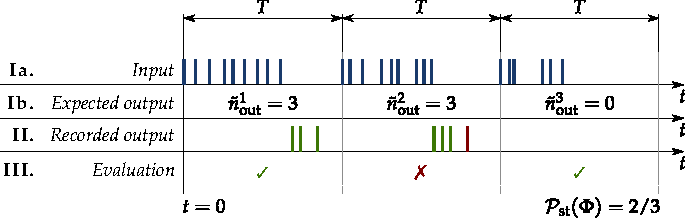
\includegraphics{media/chp4/spike_train_measure_example.pdf}
	\caption[Example of a spike train evaluation]{Example of a spike train evaluation. Bold vertical lines represent single input/output spikes. Row \emph{Ia} shows the input spike train, separated into $\Ngroups = 3$ compartments generated according to the group descriptors shown in \vref{tbl:experiment_descriptors_example}, a burst size of three and a group length $T$. Row \emph{Ib} shows the number of expected output spikes for each experiment group. Row \emph{II} depicts an examplatory result from a neuron. Accordance of the actual result with the actual result is illustrated in row \emph{III}.}
	\label{fig:spike_train_measure_example}
\end{figure}

The spike train measure is a flexible, empirical approach to single neuron evaluation. It allows to test whether a neuron with parameters \nParams responds as expected to certain inputs. As shown in \cref{fig:spike_train_measure_example}, the measure is separated into three stages. First, an input spike train, separated into \Ngroups experiment groups of length \timeWindow, is constructed. The assembly of each group follows a group descriptor, which is randomly chosen from a descriptor pool. The descriptor specifies the expected output spike count and the number of excitatory and inhibitory input bursts. In the second step the input is fed into a single neuron simulation with parameters \nParams. In the third step the recorded output spike train is evaluated with respect to the expected spike count for each compartment, resulting in an estimated probability \PST of the neuron to fulfil the behaviour encoded in the group descriptors.

Generally, the measure can be used to examine the functionality of a single neuron in an arbitrary feed-forward network. With an appropriate pool of descriptors, it can be configured to test the \BiNAM threshold condition, and implicitly the reset condition (\cref{sec:required_neuron_behaviour}). For large \Ngroups, it serves as a reliable prediction of network behaviour and provides ground-truth data for the \enquote{single group} methods introduced in \cref{sec:sgso_measure,sec:sgmo_measure}.

\subsection{Descriptor and input spike train generation}

\begin{table}
	\centering
	\small
	\begin{tabular}{r p{10.4cm}}
		\toprule
		\multicolumn{2}{c}{\spacedlowsmallcaps{Spike Train Measure Meta-Parameters}} \\

		\midrule
		\multicolumn{2}{c}{\slshape Global parameters} \\
		\midrule
		\Ngroups & Total number of experiment groups in the input spike train. Due to the random sampling performed in the method, a larger number of experiment groups results in a more accurate the result. Unless noted differently \Ngroups is chosen as 100 in this thesis.\\[0.5em]

		\midrule
		\multicolumn{2}{c}{\slshape Experiment group descriptor parameters} \\
		\midrule

		\nE & Number of excitatory input bursts. \\[0.5em]
		\nI & Number of inhibitory input bursts. Inhibitory input bursts could be used in conjunction with more sophisticated networks.\\[0.5em]
		\nOut & Number of expected output spikes. \\[0.5em]
		\wE & Weight factor of the excitatory input bursts, allows to simulate a larger synaptic weight for the excitatory synapse. Usually set to $1.0$. \\[0.5em]
		\wI & Weight factor of the inhibitory input bursts. Set to $1.0$.\\
		\bottomrule
	\end{tabular}
	\caption[Spike train evaluation method meta-parameter list]{Full list of meta-parameters in the \enquote{spike train} evaluation method.}
	\label{tbl:spike_train_measure_meta}
\end{table}

\marginnote{It is important to distinguish the number of spikes and bursts. The expected output \nOut is measured in spikes, the input in bursts (each counting \burstSizeIn spikes).}
The compartments of the randomly generated input spike train \tIn with annotated weights \wIn are generated according to a pool of experiment group descriptors. The group descriptors specify the number of excitatory and inhibitory input bursts \nE and \nI, as well as the number of expected output spikes \nOut. Individual input bursts are generated according to the data encoding parameters in \cref{sec:input_data_parametrisation,tbl:input_data_parametrisation}. Note that the input bursts in a spike train compartment are not time-sequential -- they are fused, emulating the coincidental arrival of single input bursts at \nE excitatory and \nI inhibitory synapses of a neuron (\cref{fig:fusion_model,sec:single_neuron_evaluation}). Time offsets of single spikes are solely controlled by the data encoding parameters \jitter, \jitterOffs and \isi. The annotated weights in \wIn are selected according to the specified synapse weight \wsyn with superimposed Gaussian noise according to the noise parameter \jitterWSyn. The group descriptor parameters \wE and \wI allow to rescale the weights for individual groups. The experiment group descriptors are summarised in  \cref{tbl:spike_train_measure_meta}.

\margintbl{Group descriptor example}{\centering
\begin{tabular}{r r r}
\nE & \nI & \nOut \\
\midrule
2 & 0 & 0 \\
3 & 0 & 1
\end{tabular}}{Example of group descriptors testing the threshold behaviour for $\nOnesIn = 3$, $\populationSize = 1$ and $\burstSizeOut = 1$.}{\label{tbl:experiment_descriptors_example}}
Embedding the \BiNAM threshold condition into the spike train measure framework requires two experiment group descriptors, one with $\nE = \nOnesIn \cdot \populationSize$ and an expected output spike count of $\nOut = \burstSizeOut$, and one with $\nE = (\nOnesIn - 1) \cdot \populationSize$ and $\nOut = 0$. An example is given in \cref{tbl:experiment_descriptors_example}. As the \Ngroups experiments are randomly sampled from these two descriptors and temporarily multiplexed with an interval \timeWindow into a single input spike train, the reset condition is implicitly tested -- if it was not fulfilled, the individual experiments would influence each other and the neuron would not produce the expected result.

\subsection{Evaluation}

Given the input $(\tIn, \wIn)$, the behaviour of a single neuron with parameters \nParams is simulated and the output spike train \tOut is recorded. Let \nOutI denote the expected number of output spikes for group $i$ and
\begin{align}
	\nOutAI = |\{ \tOutJ \mid \timeWindow \cdot (i - 1) \leq \tOutJ < \timeWindow \cdot i \}|
\end{align}
denote the number of actual output spikes in the $i$-th spike train compartment. The evaluation measure \PST is then defined as ratio of successful experiments to the total number of experiments:
\begin{align}
	\PSTi(\nParams) &= \begin{cases}
	          1 & \text{if } \nOutI = \nOutAI(\nParams) \\
	          0 & \text{otherwise} \\
	         \end{cases} \\
	\PST(\nParams) &= \frac{1}{\Ngroups} \cdot \sum_{i = 1}^{\Ngroups} \PSTi(\nParams)
	\label{eqn:spike_train_measure}
\end{align}
For large \Ngroups the target function $\PST(\nParams)$ can be interpreted as the probability of the neuron with parameters \nParams to exhibit the behaviour described in the experiment group descriptor pool.

\section{Approach 2: single group, single output spike}
\label{sec:sgso_measure}

The just presented spike train measure \PST has major drawbacks: $\PST(\Ngroups)$ is a discrete step function, which hinders automated, gradient based optimisation, and depending on the magnitude of the noise parameters, the number of randomly generated experiment groups \Ngroups must be rather large to produce stable and exact output values. This potentially results in long simulation times, which mitigates the promised benefit of single neuron evaluations.

\marginnote{The \enquote{single group} part of the name stems from each independent simulation run to correspond to an experiment with a single group in the spike train measure.}
This section presents the \enquote{single group, single output spike} (\SGSO) measure, which performs a limited number of independent experiments and calculates a smooth compound measure \PSGSO for the special case that the number of output spikes encoding a \enquote{one} is exactly one. In the following, we discuss the general idea, describe the input spike trains used in the experiments, the equations for \PSGSO, and finally focus on the notion of the \enquote{effective threshold potential} \EThEff.

\subsection{Concept}
\label{sec:sgso_measure_idea}

\begin{figure}
	\centering
	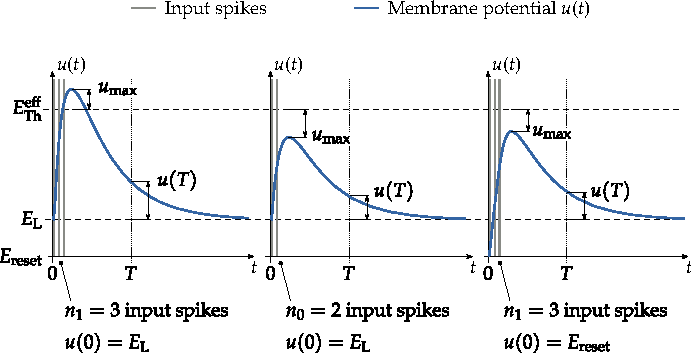
\includegraphics{media/chp4/single_group_eval.pdf}
	\caption[Conceptual overview of the single group, single output spike measure]{Conceptual overview of the single group, single output spike measure. Three independent experiments are conducted, in which a neuron with deactivated spiking mechanism is either presented \threshZero or \threshOne input spikes. The degree to which the neuron fulfils the threshold condition is determined by comparing the maximum membrane potential \umax to the effective threshold potential \EThEff. The neuron state at time \timeWindow determines how well it fulfils the reset condition.}
	\label{fig:single_group_eval}
\end{figure}

The central idea of the \SGSO measure is to analyse the distance between the maximum neuron membrane potential \umax and the effective threshold potential \EThEff. The latter is defined as the membrane potential that has to be surpassed for the neuron to inevitably generate an output spike. For single output spikes, the \BiNAM threshold condition is fulfilled if \umax reaches \EThEff for $\threshOne$ input spikes, but stays below the threshold for $\threshZero$ input spikes (\cref{eqn:threshold_condition}). In either case, there should be a large margin between \umax and \EThEff to increase robustness. The limitation to a single output spike is enforced by repeating the experiment for \threshOne input spikes with $\um(0) = \Ereset$ and $t_\mathrm{spike} = 0$. This puts the neuron into the refractory period and mimics the neuronal state following an output spike. Given these initial conditions, the neuron should not reach the threshold. The \BiNAM reset condition is tested by capturing the neuron state in all three experiments at the time \timeWindow and comparing the result to the initial neuron state. The method is sketched in \cref{fig:single_group_eval}.

\marginnote{Deactivation of the spiking mechanism is the actual reason why the measure can only handle a single output spike. Expansions of the measure allowing multiple output spikes by running follow-up experiments which restarted the simulation at the threshold-crossing point did not result in a satisfactorily smooth measure.}
A major challenge of this methodology is that -- by definition -- the neuron issues an output spike as soon as \EThEff is reached. As a result, it would hold $\umax = \ETh$. This impedes a quantification of \emph{how much} the neuron surpasses the threshold, which in return hinders the goal to optimise for a large margin and to provide a smooth evaluation measure. The pragmatic solution to the problem is to simply deactivate the neuron spiking mechanism. In the context of the \LIF model, the neuron must not reset once \ETh is reached. For the \AdEx model, the exponential spike generation current must furthermore be limited to
\begin{align}
	\ITh'(\um) = \min\{\ITh(\um), \ITh(\EThEff)\} \,.
\end{align}
This prevents the membrane potential from rising to infinity but does not obstruct neuron dynamics below the threshold.

\subsection{Deterministic input spike train generation}
\label{sec:deterministic_input_spike_train}

\begin{figure}
	\small
	\centering
	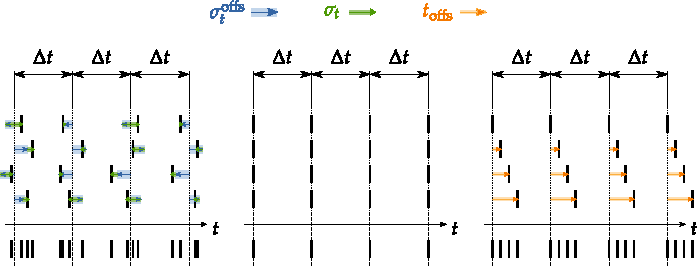
\includegraphics[trim=0cm 4cm 0cm 0cm,clip]{media/chp4/equidistant_noise.pdf}\\
	\subbottom[No noise]{%
		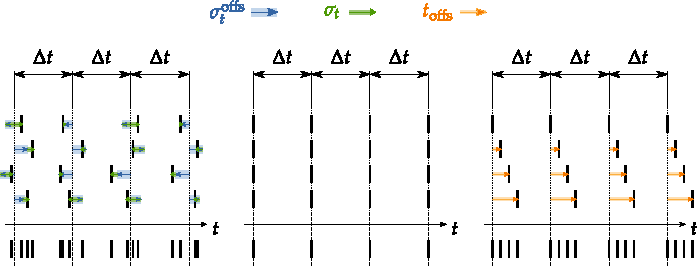
\includegraphics[trim=4cm 0cm 4cm 0.5cm,clip]{media/chp4/equidistant_noise.pdf}
		\label{fig:equidistant_noise_b}
	}%
	\subbottom[Random bursts]{%
		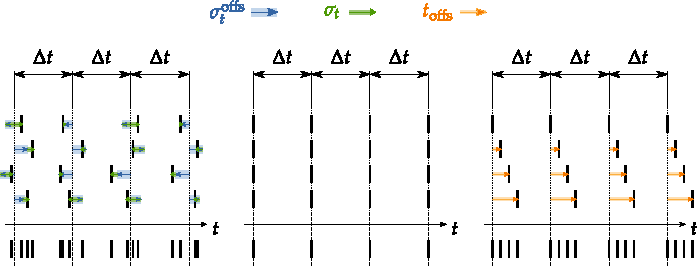
\includegraphics[trim=0cm 0cm 7.9cm 0.5cm,clip]{media/chp4/equidistant_noise.pdf}
		\label{fig:equidistant_noise_a}
	}%
	\subbottom[Equidistant offset]{%
		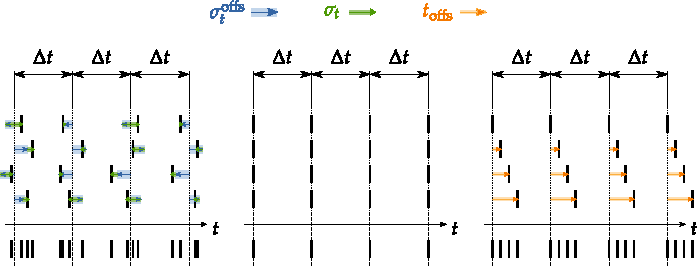
\includegraphics[trim=7.9cm 0cm 0cm 0.5cm,clip]{media/chp4/equidistant_noise.pdf}
		\label{fig:equidistant_noise_c}
	}%
	\caption[Comparison of single neuron simulation spike train generation methods]{Comparison of single neuron simulation spike train generation methods. The three sketches show four bursts each (top) which are fused into a single spike train for single neuron simulation (bottom). (a) shows four bursts generated without noise and an interspike interval \isi. The $i$-th spike of each burst is at exactly the same time. (b) shows bursts randomly generated according to the parameters \jitter and \jitterOffs as specified in \cref{sec:input_data_parametrisation}. The resulting spike packets of the fused spike trains show a certain spread. (c) deterministically emulates the spread of the spike packets by offsetting each burst by a multiple of $t_\mathrm{offs}$.}
	\label{fig:equidistant_noise}
\end{figure}

A further distinguishing goal of the \SGSO measure is determinism. Until now, input spike train generation is based on a stochastic model with noise parameters \jitter and \jitterOffs. As shown in \cref{fig:equidistant_noise_b}, determinism could be enforced by setting the spike time noise parameters \jitter and \jitterOffs to zero. Statistically, such a spike train would correspond to averaging the spike times over an infinite number of randomly generated spike trains. However, this does not account for the \jitter- and \jitterOffs-induced spread of spike times encountered when fusing multiple random bursts in a single spike train -- see \cref{fig:equidistant_noise_a}. This spread can be emulated by adding a multiple of a constant offset $t_\mathrm{offs}$ to each burst in the input spike train. The offset is chosen as
\begin{align}
	t_\mathrm{offs} = \frac{2 \cdot (\jitter + \jitterOffs)}{n_\mathrm{bursts}} \,,
\end{align}
where the denominator $n_\mathrm{bursts}$ is the number of input bursts (either $\nOnesIn$ or $\nOnesIn - 1$), and the numerator $2 \cdot (\jitter + \jitterOffs)$ the width of the $68.2\%$-quantile of the Gaussian distribution resulting from additive superposition of the Gaussian distributions accounting for \jitter and \jitterOffs. \cref{fig:equidistant_noise_c} sketches the effect of the equidistant offset.

\subsection{Evaluation measure}
\begin{figure}
	\small
	\centering
	\subbottom[Heavy-tailed sigmoids for varying $\tau$]{%
		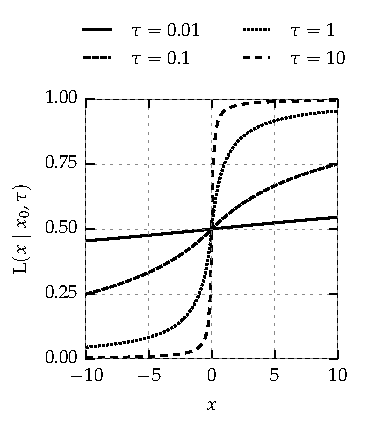
\includegraphics{media/chp4/long_tail_sigmoid_1.pdf}%
		\label{fig:long_tail_sigmoid_1}%
	}%
	\subbottom[Illustration for the calculation of $p_\mathrm{th}$]{%
		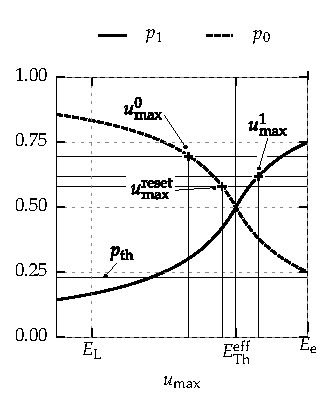
\includegraphics{media/chp4/long_tail_sigmoid_2.pdf}%
		\label{fig:long_tail_sigmoid_2}%
	}%
	\caption[Examples of heavy-tailed sigmoids and the threshold evaluation]{Examples of heavy-tailed sigmoids and the threshold evaluation. (a) shows examples of the heavy-tailed sigmoid function in \cref{eqn:logistic} with $x_0 = 0$. In contrast to other sigmoid functions, the heavy-tailed sigmoid shows no exponential falloff. (b) visualises the calculation of $p_\mathrm{th}$ in \cref{eqn:pth} for given $u_\mathrm{max}^{1}$, $u_\mathrm{max}^{0}$ and $u_\mathrm{max}^\mathrm{reset}$. The measure $p_\mathrm{th}$ results from the multiplication of the values read off the sigmoids.}
\end{figure}
\marginnote{The free parameter $\tau$ in \cref{eqn:logistic} controls the slope of sigmoid function and consequently the \enquote{softness} of $p_\mathrm{th}$. $\tau$ is chosen according to
\begin{align*}
	\tau = \frac{1 - 2 \cdot \Delta p}{2 \cdot \Delta u \cdot \Delta p} \,,
\end{align*}
where $\Delta p$ is the value of $\mathrm{L}$ at $-\Delta u$. Here these two values are $\Delta u = 2\cdot10^{-3}$ and $\Delta p = 0.2$.}
With idea and input generation laid out, we proceed to the equations specifying \PSGSO. Let $u_\mathrm{max}^{1}$, $u_\mathrm{max}^{0}$ denote the maximum membrane potentials encountered in a single neuron simulation for \nOnesIn and $\nOnesIn - 1$ input bursts respectively. The third potential $u_\mathrm{max}^\mathrm{reset}$ denotes the maximum membrane potential for \nOnesIn input bursts with the neuron starting in its refractory state. Let $\mathrm{L}(x \mid x_0)$ denote a heavy-tailed sigmoid function
\begin{align}
	\mathrm{L}(x \mid x_0) &= \frac{1}2 \cdot \left( 1 + \frac{\tau \cdot (x - x_0)}{1 + \tau \cdot |(x - x_0)|} \right) \,.
	\label{eqn:logistic}
\end{align}
An important property of $\mathrm{L}(x \mid x_0)$ is its non-exponential falloff, causing the sigmoid to saturate slowly. Goal of this choice is to facilitate parameter optimisation by providing a distinct gradient. Example plots of $\mathrm{L}(x \mid x_0)$ are shown in \cref{fig:long_tail_sigmoid_1}. The first ingredient to the evaluation measure, $p_\mathrm{th}$, describes accordance with the threshold condition
\begin{align}
	p_\mathrm{th} &= \mathrm{L}(u_\mathrm{max}^{1} \mid \EThEff) \cdot (1 - \mathrm{L}(u_\mathrm{max}^{0} \mid \EThEff)) \cdot (1 - \mathrm{L}(u_\mathrm{max}^\mathrm{reset} \mid \EThEff)).
	\label{eqn:pth}
\end{align}
\cref{fig:long_tail_sigmoid_2} sketches the individual factors of the above equation for fixed potentials. Large $u_\mathrm{max}^{1}$, and small $u_\mathrm{max}^{0}$ and $u_\mathrm{max}^\mathrm{reset}$ result in a high valuation in the compound measure $p_\mathrm{th}$.

The final ingredient to the measure is an estimation of how well the reset condition is fulfilled. Let $\vec v^{1}_T$, $\vec v^{0}_T$ and $\vec v^\mathrm{reset}_T$ denote neuron state vector of the corresponding simulation runs at time \timeWindow, and \nStateI the initial neuron state. Accordance with the reset condition $p_\mathrm{reset}$ is measured as
\begin{align}
	p_\mathrm{reset} = \exp \left(- \| \vec v^{1}_T - \nStateI \| - \| \vec v^{0}_T - \nStateI \| - \| \vec v^\mathrm{reset}_T - \nStateI \|)\right) \,.
	\label{eqn:preset}
\end{align}
The norm $\|\cdot\|$ should be chosen such that individual vector dimensions are rescaled to similar value ranges. The final evaluation measure $\PSGSO(\nParams)$ for a parameter vector \nParams is defined as
\begin{align}
	\PSGSO(\nParams) = p_\mathrm{th}(\nParams)  \cdot p_\mathrm{reset}(\nParams)  \,.
	\label{eqn:psgso}
\end{align}

\subsection{Effective threshold potential}
\label{sec:effective_threshold_potential}

The effective threshold potential \EThEff is defined as the membrane potential at which a neuron inevitably produces an output spike (\cref{sec:sgso_measure_idea}). For the \LIF model, it trivially holds $\EThEff = \ETh$. For the \AdEx measure, \EThEff corresponds to the unstable stationary point in the membrane potential bifurcation analysis (\cref{fig:eif_state}). Consider the exponential current \ITh in the \AdEx model (\cref{eqn:adex_ith})
\begin{align}
	\ITh = \Gl \cdot \DT \cdot \exp\left((\um(t) - \EThExp) \cdot \DT^{-1}\right)\,.
\end{align}
\marginnote{As discussed in \cref{sec:parameter_normalisation}, the leak potential is only an offset to all membrane potentials.}
For an absence of inhibitory currents ($\iadap(t) \leq 0$ and $\Gi(t) = 0$), and a leak potential $\El = 0$, $\EThEff$ is given as the membrane potential $x$ at which leak and threshold current cancel each other out
\begin{align}
	\Gl \cdot x &= \Gl \cdot \DT \cdot \exp\left( (x - \EThExp) \cdot \DT^{-1} \right) \,.
	\label{eqn:etheff_base}
\end{align}
We now discuss two ways in which the equation can be solved for $x$.

\paragraph{Lambert $W$ function}
\marginnote{The Lambert $W$ function is defined as\\
$W(z) = X(x) \Leftrightarrow $\\
$z = X(x) \cdot \exp(X(x))$\\
with a real-valued result if $z > -\frac{1}e$ holds.}
Rearranging \cref{eqn:etheff_base} yields
\begin{align}
	\DT &= x \cdot \exp\left(- (x - \EThExp) \cdot \DT^{-1} \right) \notag\\
	\Leftrightarrow - \exp\left(- \EThExp \cdot \DT^{-1} \right) &= - x \cdot \DT^{-1}  \cdot \exp\left(- x \cdot \DT^{-1} \right) \,.
\end{align}
This equation can be solved with the Lambert $W$ function \cite{corless1996lambertw}
\begin{align}
	\EThEff = x = - \DT \cdot W\left(- \exp\left(- \EThExp \cdot \DT^{-1} \right) \right) \,.
\end{align}
$W(z)$ possesses a real-valued solution for $z > -\frac{1}{e}$. It must hold
\begin{align}
	\exp\left(- \EThEff \cdot \DT^{-1} \right) < \exp(-1) \Leftrightarrow \EThEff &> \DT \,.
\end{align}
For $\EThEff \leq \DT$ the threshold current \ITh would always be larger than the leak current. The neuron would be in an unstable state in which it repeatedly generates output spikes.

\paragraph{Iterative calculation}
\marginnote{Newton's method is likely to diverge if the logarithm is not applied, as the derivative still contains an exponential function.}
For a practical implementation of the calculation of \EThEff without the Lambert $W$ function, \cref{eqn:etheff_base} can be solved iteratively using Newton's method. However, it is important to apply the logarithm to the equation
\begin{align}
	f \left(x\right) = 0 &= \log\left(\DT\right) + (x - \ETh) \cdot \DT^{-1} - \log\left(x\right) \,.
\end{align}
The iterative solution is given as
\begin{align}
	x_0 &= \ETh \,,\\
	x_{n + 1} &= x_{n} - \frac{f\left(x_{n}\right)}{f'\left(x_{n}\right)}
		= x_{n} -
			\frac{\log\left(\DT\right) + (x - \ETh) \cdot \DT^{-1} - \log\left(x\right)}
			{\DT^{-1} - x^{-1}}\notag\,,
\end{align}
where $\ETh > 0$ and $\DT > 0$. Under these circumstances the formula usually converges to a solution with an accuracy of $\SI{1}{\nano\volt}$ in three to four steps.

\section{Approach 3: single group, multiple output spikes}
\label{sec:sgmo_measure}

In contrast to the spike train measure, the \SGSO measure produces a smooth, non-discrete output. Yet, the former accurately models the environment of a single neuron in a \BiNAM network which receives a new sample in an interval \timeWindow. Furthermore, all properties of the neuron are tested, including the spiking mechanism, refractory period and the adaptation mechanism, and there is no limitation regarding the number of output spikes.

Combining the advantageous properties of the previous two measures is the goal of the \enquote{single group, multiple output spikes} measure (\SGMO). It aims at respecting all neuron model characteristics, allowing for an arbitrary expected output spike number, while still being computationally inexpensive and guaranteeing a smooth evaluation measure. \cref{sec:sgmo_measure_idea} presents the general idea on how to tackle the lofty goals mentioned above. It furthermore provides the defining equations of the measure, which assume the existence of a \emph{fractional spike count} \qOutA. An efficient algorithm for the calculation of the said \qOutA is covered in the second part, \cref{sec:sgmo_measure_fractional_spike_count}.

\subsection{General idea}
\label{sec:sgmo_measure_idea}

Again, the overall goal of the measure is to facilitate neuron parameter optimisation with respect to the threshold and reset conditions (\cref{sec:required_neuron_behaviour}). Optimisation of the threshold condition can be formulated as minimisation of the error $E$ in the following framework
\begin{align}
	E(\nParams) = | \nOut - \nOutA(\nParams, t^\mathrm{in}_1) | + \nOutA(\nParams, t^\mathrm{in}_0)\,,
\end{align}
where $t^\mathrm{in}_1$ and $t^\mathrm{in}_0$ are deterministic input spike trains (\cref{sec:deterministic_input_spike_train}) for which the neuron is expected to produce \nOut and zero output spikes respectively. An eminent disadvantage of the above equation are the discrete spike counts $\nOutA$, which cause the error function $E(\nParams)$ to take the form of a step function.

\marginnote{A fractional output spike count $\qOutA = 3.5$ should for example be interpreted as \enquote{the neuron outputs three spikes, and is already half way to generating a fourth spike}.}
The crucial idea is to replace discrete spike counts \nOutA with fractional spike counts $\qOutA \in \R^+$, which encode both the integral number of output spikes \nOutA, as well as the estimated likelihood of another output spike \pOutA. Assuming the existence of such a measure \qOutA, the error equation can be reformulated as
\begin{align}
	E(\nParams) = | \sgmoOffs + \nOut - \qOutA(\nParams, t^\mathrm{in}_1) | + \qOutA(\nParams, t^\mathrm{in}_0)\,,
\end{align}
where the offset \sgmoOffs should theoretically be chosen as $\sgmoOffs = \nicefrac{1}2$ to maximise the margin between two discrete spike count steps: the neuron should not be close to issuing $\nOut - 1$ spikes, but also not too close to issuing $\nOut + 1$ spikes. In case \qOutA is not linear with respect to the variation of a single parameter dimension, another choice of \sgmoOffs might yield a more robust behaviour. The value chosen here is $\sgmoOffs = 0.3$.

\begin{figure}
	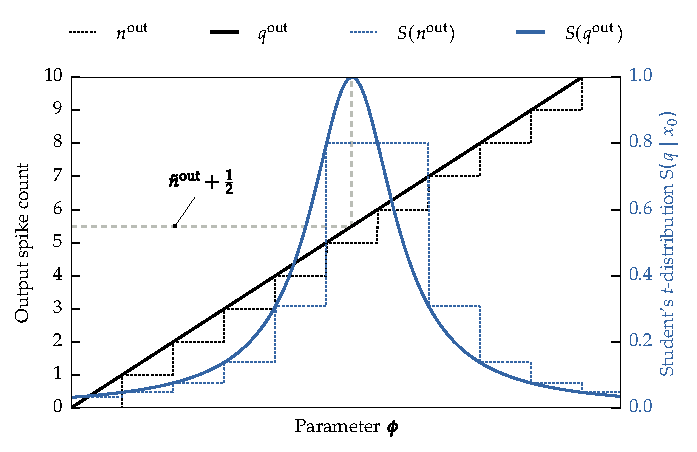
\includegraphics{media/chp4/student_t_step.pdf}
	\caption[{Idealised sketch of the SGMO measure}]{Idealised sketch of the \SGMO measure. The output spike count $\nOutA(\phi)$ over a neuron parameter $\phi$ is smoothed to a fractional spike count measure $\qOutA(\phi)$ (here in its ideal linear form). The fractional spike count is converted to a bell-shaped function (an unnormalised Student's $t$-distribution) with zero to one value range, which indicates how well the current spike count matches the target spike count $\nOut$.}
	\label{fig:student_t_step}
\end{figure}
\marginnote{As with the previous evaluation measure, the semantic value of the pseudo-probabilities is fairly limited in a mathematical sense and should be seen as a normalisation only.}
The additive error value $E(\nParams)$ is rewritten as pseudo-probabilistic value $p_\mathrm{th}(\nParams)$ consisting of the product of two unnormalised, bell-shaped Student's $t$-distributions with parameter $\nu = 1$ (also known as Cauchy distribution), which measure how close \qOutA is to \nOutA for input $t^\mathrm{in}_1$ (sketched in \cref{fig:student_t_step}) and how close to zero for input $t^\mathrm{in}_0$
\begin{align}
	p_\mathrm{th}(\nParams) &= \frac{1}{1 + \big(\sgmoOffs + \nOut - \qOutA(\nParams, t^\mathrm{in}_1)\big)^2} \cdot \frac{1}{1 + \big(\qOutA(\nParams, t^\mathrm{in}_0)\big)^2} \,.
	\label{eqn:sgmo_pth}
\end{align}
Analogue to similar considerations in the \SGSO measure, the use of a heavy-tailed bell-shaped function ensures non-zero $p_\mathrm{th}(\nParams)$ with a distinct gradient over vast regions of the parameter space. This gradient might be sufficient to guide an automated parameter optimiser through the neuron parameter space.

The final ingredient to the measure is an estimation of how well the reset condition is fulfilled. Here, the same approach as in the \SGSO spike measure in \cref{eqn:preset} is employed
\begin{align}
	p_\mathrm{reset}(\nParams) = \exp(-\|\vec v^1_T - \nStateI \|)\,,
\end{align}
where $\vec v^1_T$ is the state of the neuron at time \timeWindow for input $t^\mathrm{in}_1$ and \nStateI is the initial neuron state. Again, the norm $\|\cdot\|$ should rescale the individual state vector components to a comparable value range. The resulting evaluation measure value $\PSGMO(\nParams)$ is given as
\begin{align}
	\PSGMO(\nParams) = p_\mathrm{th}(\nParams) \cdot p_\mathrm{reset}(\nParams) \,.
\end{align}

\subsection{Fractional spike count}
\label{sec:sgmo_measure_fractional_spike_count}

\marginnote{To tighten the notation, the spike train descriptor \tIn is not explicitly denoted. Of course, a spike train descriptor must nonetheless be passed to the underlying single neuron simulation.}
With the basics of the single group, multiple output spike measure in place, we are ready to address the fractional spike count measure $\qOutA(\nParams)$ itself. This section first presents a widely unsuccessful approach to the calculation of the fractional spike count. The lessons learned are then incorporated into the construction of a more robust measure. Yet, before we begin, a more thorough definition of the semantics of the seemingly paradoxical \enquote{fractional spike count} is appropriate.

\paragraph{Properties of the fractional spike count}
\marginfig{Sketch of the fractional spike count decomposition}{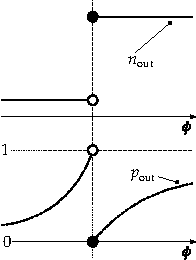
\includegraphics{media/chp4/pout.pdf}}{Sketch of the fractional spike count decomposition. The fractional spike count measure smoothly interpolates between the discrete steps in \nOutA (top graph) by adding a fractional value \pOutA (bottom graph), which is zero right at the point at which an additional output spike is generated and close to one immediately previous to that point.}{\label{fig:pout}}
For the sake of simplicity, let us consider a single variable parameter dimension with value \nParam. All other parameters in the parameter vector \nParams should assumed to be constant. Of course, the same concepts apply to more than one variable parameter dimension, yet this would be harder to visualise and requires more elaborate mathematical notation. Furthermore, the postulated properties may be slightly violated by the actually selected fractional spike count measure. They are mere guidelines towards designing such a measure.

The defining property of $\qOutA(\nParam)$ is its decomposability into the discrete spike count $\nOutA(\nParam) \in \N$ and an additive fractional part $\pOutA(\nParam) \in [0, 1)\subset \R$. The latter can be interpreted as the likelihood of an additional spike, which smoothly interpolates between the steps of its discrete counterpart
\begin{align}
	\qOutA(\nParam) = \nOutA(\nParam) + \pOutA(\nParam) \,.
	\label{eqn:fsc_decomposition}
\end{align}
Given an infinitesimally small $\epsilon \to 0$, the fractional $\pOutA(\nParam)$ should fulfil the following conditions
\begin{align}
	\pOutA(\nParam) = 0 &\Leftrightarrow \nOutA(\nParam) > \nOutA(\nParam - \epsilon) \vee \nOutA(\nParam) > \nOutA(\nParam + \epsilon) ,
	\label{eqn:fsc_zero}\\
	\pOutA(\nParam) \to 1 &\Leftrightarrow \nOutA(\nParam) < \nOutA(\nParam - \epsilon) \vee \nOutA(\nParam) < \nOutA(\nParam + \epsilon) ,
	\label{eqn:fsc_one}
\end{align}
or in other words, the upper corner points of the staircase \nOutA are located on the curve \pOutA (\cref{fig:pout}). In order to facilitate automatic parameter optimisation, \pOutA should be continuous and monotonous for maximally large intervals $[\check{\nParam}, \hat{\nParam}]$ with
\begin{align}
	\nOutA(\nParam) = \nOutA(\nParam') \quad \text{ where } \quad \check{\nParam} \leq \nParam, \nParam' \leq \hat{\nParam} \,.
	\label{eqn:fsc_interval}
\end{align}
With these properties in place, we discuss a simple, yet flawed method for the calculation of \pOutA.

\subsection{Minimal apical voltage difference}
The method we discuss here is based on an intriguingly simple observation, which in practice fails spectacularly. Consider two infinitesimally close parameter values $\nParam$ and $\nParam'$, with the value \nParam causing the neuron to produce an additional spike compared to $\nParam'$. Put more precisely, it holds
\begin{align}
\nOut(\nParam) - \nOut(\nParam') = 1 \quad \text{ with } |\nParam - \nParam'| \to 0 \,.
\end{align}
\marginnote{The author never encountered a situation in which the spike was not produced at the location of a local maximum. Yet, since the intricate dynamical systems are rather complex, no effort was made at proving this conjecture, so it should be taken with a grain of salt.}
Repeatedly comparing the membrane potential traces $\um(t)$ for such parameter pairs $\nParam$ and $\nParam'$ suggests that the additional spike is very likely to be produced at a time $t$ which corresponds to a local maximum in the membrane potential trace for the parameter $\nParam'$. Thus, it seems reasonable to assume that a necessary precondition for time points $t$ at which spikes may arise is $\dum(t) = 0$ and $\ddum(t) < 0$. With this thought in mind, the fractional spike count component \pOutA could be defined as follows
\begin{align}
	\pOutA = 1 - \frac{\min \{\EThEff - \um(t) \mid \dum(t) = 0 \wedge \ddum(t) < 0\}}{\EThEff - \El} \,,
	\label{eqn:mavd}
\end{align}
\marginnote{Note that due to discontinuity, the spikes themselves do not fulfil the condition $\dum(t) = 0$. They are thus filtered out.}
which expresses the normalised minimal voltage difference between the local maxima of the membrane potential and the effective threshold potential \EThEff (\cref{sec:effective_threshold_potential}). If the maximum membrane potential is close to \EThEff, it is likely that an additional spike will be introduced, and it holds $\pOutA = 1$. If the maximum membrane potential is \El, the likelihood of an additional spike is small, so  $\pOutA = 0$.

\begin{figure}
	\centering
	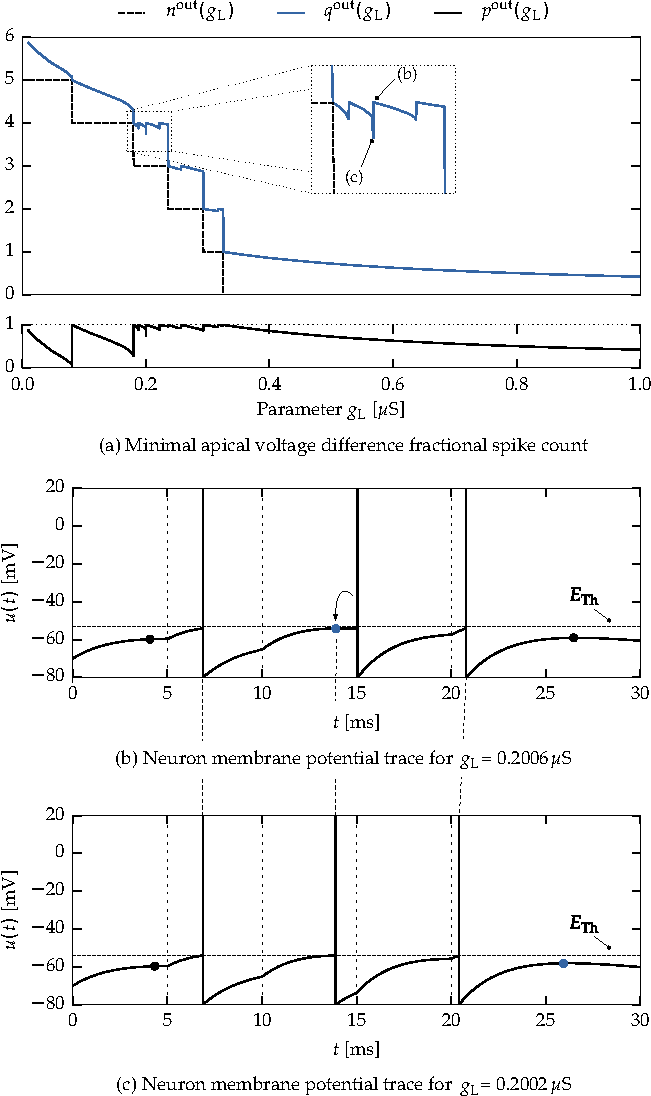
\includegraphics{media/chp4/min_apices_problems.pdf}
	\caption[Unsuccessful fractional spike count calculation strategy]{Results for the unsuccessful \enquote{minimal apical voltage difference} fractional spike count. (a) plots the number of output spikes $\nOutA(\Gl)$, the fractional spike count measure $\pOutA(\Gl)$ and the pure fractional part $\qOutA(\Gl)$, over the neuron parameter $\Gl$. The fractional spike count is calculated according to \cref{eqn:mavd}. The tested neuron is a \LIF neuron which receives five input spikes in a five millisecond interval starting at $t = 0$. As can be seen in (a), \pOutA exhibits severe discontinuities and non-monotonous behaviours. The figures (b) and (c) show the membrane potential traces $\um(t)$ for the values of $\Gl$ indicated in (a). Filled circles show the location of the local maxima. As can be seen, the discontinuity in \pOutA is caused by the second spike \enquote{jumping} to the position of the largest maximum (blue circles).}
	\label{fig:qout_unsuccessful}
\end{figure}
However, as shown in \cref{fig:qout_unsuccessful}, this idea fails on multiple levels. While a maximum in the membrane potential trace at time $t$ for a parameter $\nParam'$ might be a necessary precondition for the production of a spike for \nParam at time $t$, the reverse does not hold. Even the largest local maximum in the membrane potential trace is by no means a sufficient condition for the production of an \emph{additional} spike for any \nParam. The most spectacular failure of this assumption arises if variation of \nParam indeed produces a spike at the predicted location, but in response a spike at another location disappears.

The normalisation of \pOutA poses another problem. For the parameter value \nParam, at which a new spike has just been introduced, \cref{eqn:fsc_zero} requires \pOutA to be set to zero. In practice the largest local maximum is larger than \El, causing \pOutA to be set to a value greater than zero.

Nevertheless, the measure possesses at least one positive trait. It produces a smooth curve with subtle slope for $\nOutA(\nParam) = 0$. This is somewhat expected, since most disturbances in the neuron dynamics are generated by the output spike generation mechanism.

To summarise, it should be apparent from these examples, that running a single neuron simulation and trying to mingle some more or less arbitrarily measured membrane potentials into a single value \pOutA is doomed to fail. Explicit membrane potential measurements are neither expressive, nor properly normalisable. Thus, the next approach is based on a fundamentally different idea.

\subsection{Minimal membrane potential perturbation}
The notion of \enquote{likelihood of an additional spike} could be reformulated as \enquote{what is the minimal amount of additional energy that must be pumped into the neuron to produce another spike?}. An obvious way of injecting energy into a spiking neuron is to offset the membrane potential at a certain time $t$ by a small voltage \pum. The basic idea of the approach to the fractional spike count measure presented here is to find the minimal \pum, which introduces an additional output spike. However, two open questions remain: at which times $t$ should the perturbation take place and what is the possible value range of \pum?

Searching a minimal \pum over a dense grid of times $t$ is not a viable option, as this approach is not only slow, but would inflate the search space unnecessarily since the neuronal behaviour usually does not differ tremendously between two close points in time $t$ and $t'$. The events which influence the neuronal dynamical system the most are the output spikes themselves. The membrane potential perturbation is thus performed at the times of highest behavioural uncertainty, namely, at the beginning of the simulation, and the end of each refractory period in the original, undisturbed neuron simulation.

The possible value range for perturbations at time $t$ is limited by the original membrane potential $\um(t)$ and the effective threshold potential \EThEff. It must hold $\pum(t) \in [0, \EThEff - \um(t)]$. Given these considerations, the entire fractional spike count calculation can be expressed mathematically as
\begin{align}
	\pOutA(\nParams) &= 1 - \min\left\{ \frac{\pum}{\EThEff - \um(t + \TauRef)} \middle| n^\mathrm{out}_\mathrm{pert}(\nParams, t + \TauRef, \pum) > \nOutA(\nParams), \right. \notag\\
	&\left. \phantom{\frac{\pum}{\EThEff}} \quad \pum \in [0, \EThEff - \um(t + \TauRef)], t \in (-\TauRef) \Arrowvert \tOut \right\} \,,
	\label{eqn:mmpp}
\end{align}
\marginnote{The gist of the algorithm as a whole is captured in \cref{eqn:mmpp}. Exact descriptions of the optimised fractional spike count algorithm are out of scope for this thesis. Interested readers can find the entire implementation in the accompanying source code. For example, an especially crude trick was used for efficiently relaying $\pum$ to the neuron simulator: $t$ and $\pum$ are encoded as a special input spike with $\pum$ stored in the payload of a \enquote{NaN} weight value.}
where $n^\mathrm{out}_\mathrm{pert}(\nParams, t, \pum)$ is the output spike count for perturbation with offset \pum at time $t$, \tOut are the original output spike times, and $\um(t)$ refers to the original membrane potential trace.
% The scarcity of assumptions regarding the underlying neuron model in \cref{eqn:mmpp} is a beautiful property of this approach. It generates sound results as long as the neuron produces additional spikes if the membrane potential is artificially increased at the end of the refractory period.

Algorithmic implementations of \cref{eqn:mmpp} should take various optimisations into account. Most importantly, the search for the minimum \pum at time $t$ should be implemented as a binary search. Furthermore, since neuron dynamics only need to be simulated starting from the time-point of the perturbation $t$, the algorithm should start its minimum search at the largest $t$, and thus successively restrict the search space for longer simulation durations. The next optimisation resembles the concept of dynamic programming \cite{bellman1957dynamic}. For each tested time $t$, the neuronal states \nState which did or did not lead to an additional output spike are stored in a table. Whenever the simulator passes $t$ it compares the current neuron state to the corresponding table entry allowing for early abortion. This approach has to be implemented with great care, since all neuron states -- including for example the adaptation current $\iadap(t)$ -- influence the generation of additional output spikes.

\begin{figure}
	\small
	\centering
	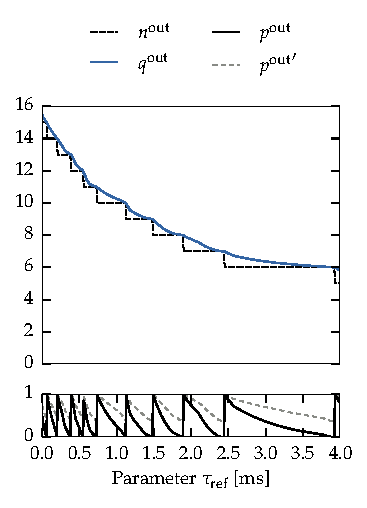
\includegraphics[trim=0cm 7.25cm 0cm 0.4cm, clip]{{media/chp4/sweep_tauRef_lif.csv}.pdf}\\%
	\subbottom[\LIF neuron, sweep $\Gl \, {[\si{\micro\siemens}]}$]{%
		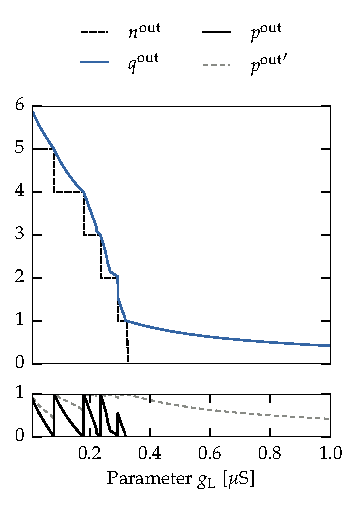
\includegraphics[trim=2.5mm 0.8cm 1mm 1.65cm, clip]{{media/chp4/sweep_gL_lif.csv}.pdf}
		\label{fig:qout_mmpp_a}
	}%
	\subbottom[\AdEx neuron, sweep $\Gl \, {[\si{\micro\siemens}]}$]{%
		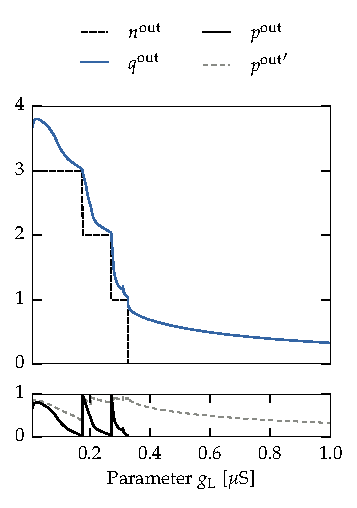
\includegraphics[trim=0cm 0.8cm 1mm 1.65cm, clip]{{media/chp4/sweep_gL_adex.csv}.pdf}%
		\label{fig:qout_mmpp_b}
	}
	\subbottom[\LIF neuron, sweep $\ETh \, {[\si{\milli\volt}]}$]{%
		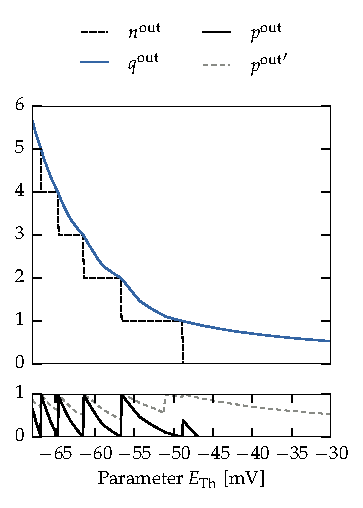
\includegraphics[trim=2.5mm 0.8cm 1mm 1.65cm, clip]{{media/chp4/sweep_eTh_lif.csv}.pdf}
		\label{fig:qout_mmpp_c}
	}%
	\subbottom[\AdEx neuron, sweep $\ETh \, {[\si{\milli\volt}]}$]{%
		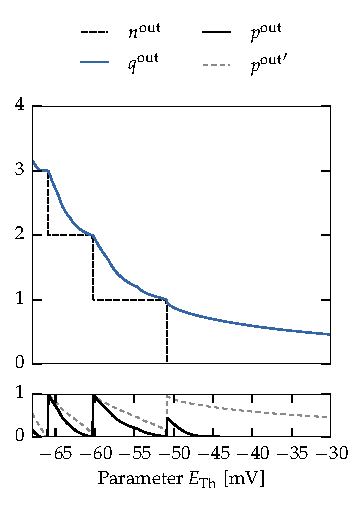
\includegraphics[trim=0cm 0.8cm 1mm 1.65cm, clip]{{media/chp4/sweep_eTh_adex.csv}.pdf}%
		\label{fig:qout_mmpp_d}
	}
	\subbottom[\LIF neuron, sweep $\TauRef \, {[\si{\milli\second}]}$]{%
		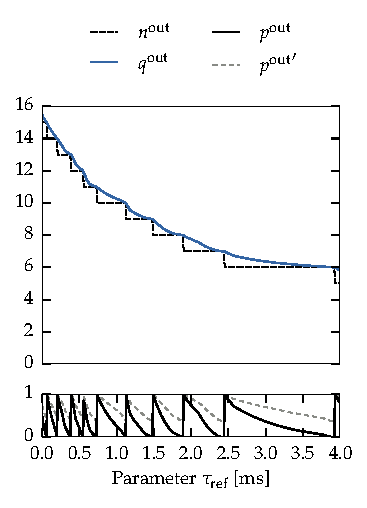
\includegraphics[trim=2.5mm 0.8cm 1mm 1.65cm, clip]{{media/chp4/sweep_tauRef_lif.csv}.pdf}
		\label{fig:qout_mmpp_e}
	}%
	\subbottom[\AdEx neuron, sweep $\TauRef \, {[\si{\milli\second}]}$]{%
		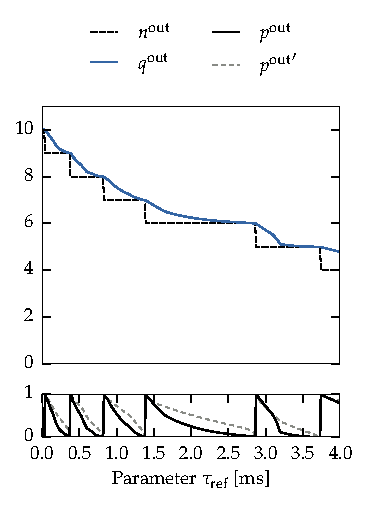
\includegraphics[trim=0cm 0.8cm 1mm 1.65cm, clip]{{media/chp4/sweep_tauRef_adex.csv}.pdf}%
		\label{fig:qout_mmpp_f}
	}%
	\caption[Minimal membrane potential perturbation measure examples]{Minimal membrane potential perturbation measure examples, comparison between \LIF (left) and \AdEx (right) neurons with sweeps over different parameter dimensions.}
	\label{fig:qout_mmpp}
\end{figure}
As shown in \cref{fig:qout_mmpp}, the perturbation-based method is clearly superior to the previous concept -- at least for regions with $\nOutA > 0$. For $\nOutA = 0$ \pOutA (black) falls very quickly to or stays at zero, as can be seen for example in the bottom portion of \cref{fig:qout_mmpp_d}. The pragmatic solution taken here is to employ the previous measure (denoted as $\pOutA'$ in the figure) in regions with $\nOutA = 0$. In combination (blue graphs, \qOutA), the two measures fulfil the behavioural constraints postulated above to a high degree. The pure fractional part of the measure \pOutA, which is mostly monotonous between steps, fills the entire range between zero and one, and touches the upper corners of the underlying step function \nOutA. Minor deficiencies concern the non-linear interpolation between the steps, the generation of plateaus as in \cref{fig:qout_mmpp_f}, and very small, non-monotonous kinks as in \cref{fig:qout_mmpp_b}. However, since an optimiser is most likely to adapt multiple dimensions concurrently, at least one gradient should point into the correct direction. Neither the plateaus, nor the occasional kink should thus present a serious problem.

\section{Neuron evaluation software framework}
\label{sec:adexpsim}

This section gives insight into the software framework and tools for single neuron evaluation experiments. Following an overview of the system architecture, the interactive parameter space exploration tool \emph{AdExpSimGui} and in particular the modular high performance neuron simulator are discussed.

\subsection{Architectural overview}

\begin{figure}
	\centering
	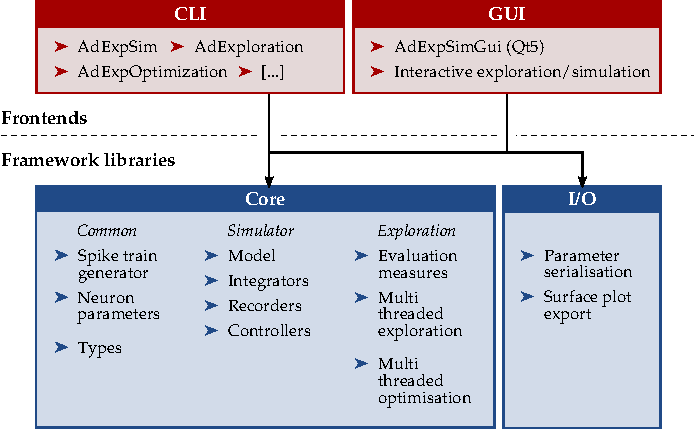
\includegraphics{media/chp4/adexpsim.pdf}
	\caption[Architectural overview of the AdExpSim framework]{Architectural overview of the \AdExpSim framework developed for this thesis with distinction between the frontend applications and the actual framework libraries, which implement the listed functionalities in a reusable manner.}
	\label{fig:adexpsim}
\end{figure}

\marginnote{The entire framework, including the \acrshort{CLI} and \acrshort{GUI} applications, amounts to more than $18\,000$ lines of code, including inline documentation. The core library is solely based on the C++ standard library and can be used on any system with a standard compliant C++14 compiler.}
The single neuron simulator and the three evaluation methods are implemented as part of the \AdExpSim framework in the C++14 programming language \cite{isocpp14}. Architecture and components of the framework are sketched in \cref{fig:adexpsim}. Low-level facilities, such as the generation of spike trains, normalisation of neuron parameters and the \acrshort{LIF} and \acrshort{AdEx} neuron model simulator, are implemented as part of a core library. On a higher abstraction level, the same library implements the neuron evaluation measures presented in the previous sections, as well as classes for multi threaded parameter sweeps (exploration) and optimisation. The input and output (I/O) library provides functions for serialisation of the user-provided parameters to \acrshort{JSON} (\acrlong{JSON}, \cite{json2014rfc}), as well as facilities for the export of exploration data as surface plots.

\subsection{Frontend applications}
\label{sec:adexpsimgui}

\begin{figure}[t]
	\small
	\centering
	\subbottom[Parameter control panel]{%
		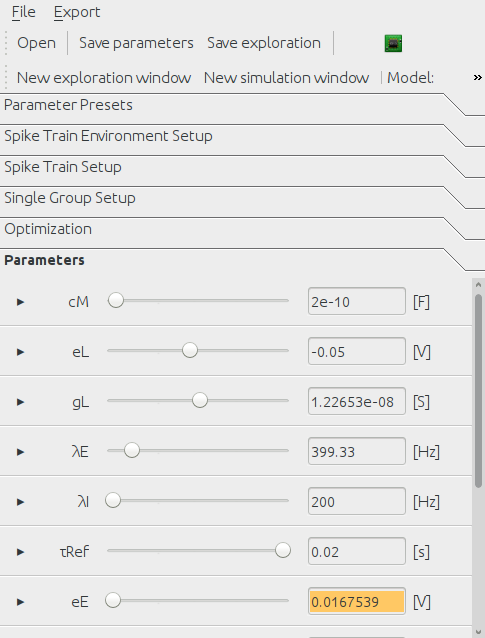
\includegraphics[height=0.235\textheight]{media/chp4/adexpsimgui_params.png}%
		\label{fig:adexpsimgui_params}%
	}~
	\subbottom[Neuron simulation view]{%
		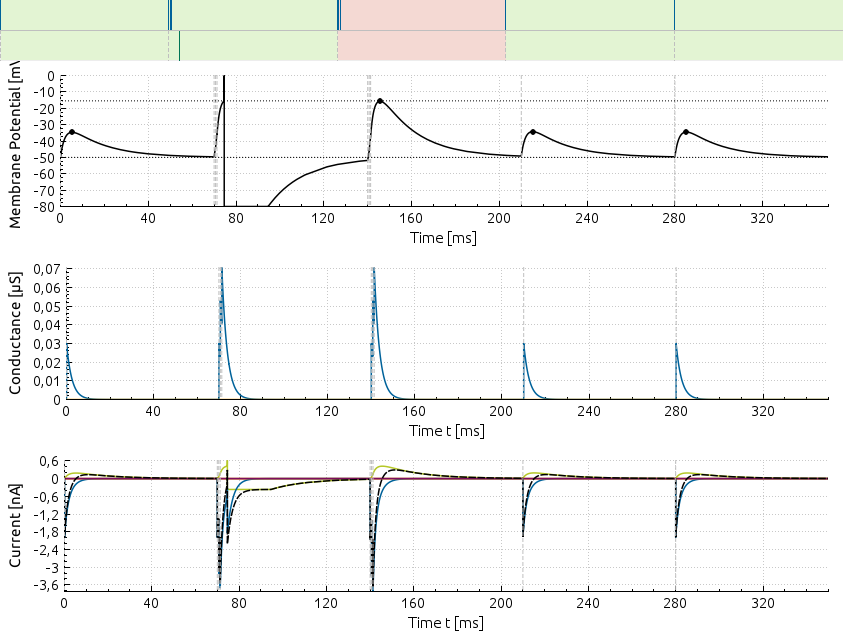
\includegraphics[height=0.235\textheight]{media/chp4/adexpsimgui_simulation.png}%
		\label{fig:adexpsimgui_simulation}%
	}
	\subbottom[Design space exploration view]{%
		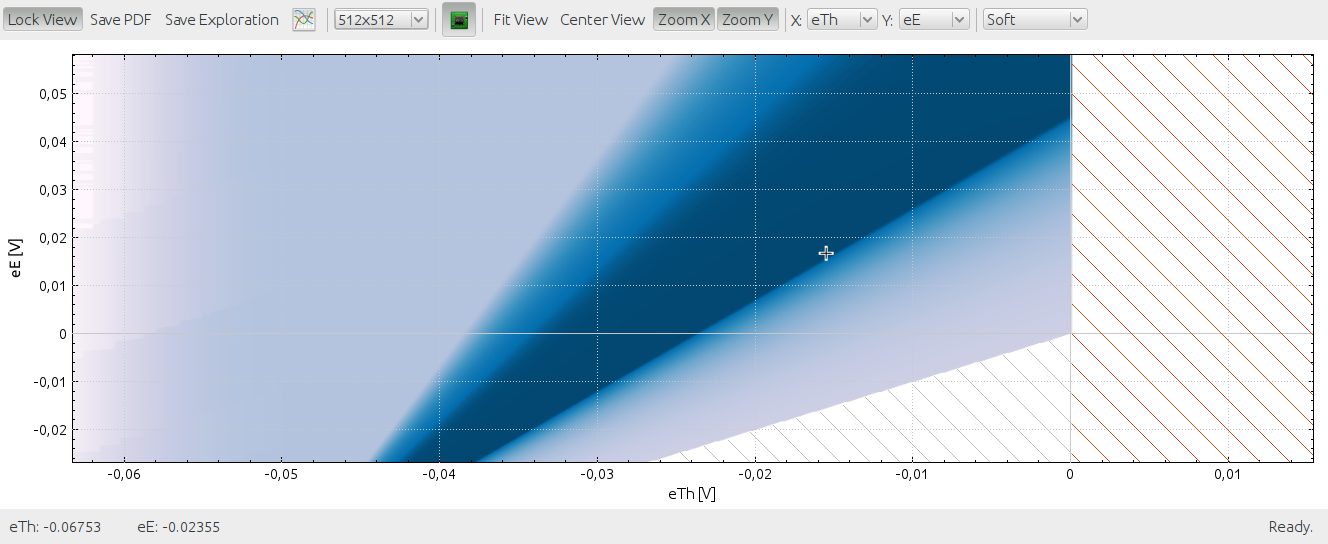
\includegraphics[width=\textwidth]{media/chp4/adexpsimgui_exploration.png}%
		\label{fig:adexpsimgui_exploration}%
	}%
	\caption[Screenshots of the AdExpSimGui tool]{Screenshots of the \emph{AdExpSimGui} tool. (a) depicts the parameter control panel, (b) shows the spike train neuron simulation window, and (c) shows a design space exploration window. Dark colours correspond to higher-rated parameters vectors, the red hatching to parameters outside the hardware range, the grey hatching to invalid parameter combinations.}
	\label{fig:adexpsimgui}
\end{figure}

The \AdExpSim framework comes with a set of frontend applications. The \acrfull{CLI} applications are too numerous to list in their entirety, but are usually thin wrappers around the core library which expose an individual aspect of the core functionality to end users. These programs require no interaction and facilitate batch processing of exploration and optimisation tasks. Most of the programs are designed to run a specific experiment and can be configured directly in the source code.

The \emph{AdExpSimGui} \acrfull{GUI} application is an interactive tool for design space exploration. The application itself is based on the \emph{Qt5} application framework and the \emph{QCustomPlot} plotting library \cite{qt5,qcustomplot}. The control panel shown in \cref{fig:adexpsimgui_params} allows users to setup neuron and evaluation measure parameters. Results of a spike train evaluation for the current parameter vector, along with the corresponding neuron voltage, conductance and current traces are displayed in the simulation window depicted in \cref{fig:adexpsimgui_simulation}. Two dimensional projections of the high-dimensional neuron parameter space can be viewed in one or multiple exploration windows (\cref{fig:adexpsimgui_exploration}). The user can interactively pan and zoom the design space, and select the evaluation measure and the design space dimensions. Changes to the neuron parameters are reflected in all exploration windows at the same time. The exploration view highlights invalid parameter combinations and parameters outside the range supported by \NMPM.

\subsection{High performance single neuron simulator}
\label{sec:simulator}

The demands regarding the functionality of the high performance single neuron simulator at the core of the \AdExpSim framework vary greatly between the individual evaluation measures. An incomplete list of features includes the recording of voltage, current and conductance traces, the tracking of local maxima, early abortion, simulation of both the \acrshort{AdEx} and \acrshort{LIF} models, usage of various integrators, deactivation of the spiking mechanism, as well as injection of perturbation voltages at defined times. To this end, the simulator is implemented as a C++ template. This allows building individual simulator instances tailored specifically to a feature set. The compiler can optimise each instance to a high-performance and cache-oblivious loop consisting of a few hundred assembler instructions. See \cref{app:simulator_code} for technical details.

\pagebreak


\section{Evaluation method comparison}
\label{sec:single_neuron_measure_comparison}

This section aims at providing a direct comparison of the three evaluation measures. First, the expected properties of the measures are summarised. Then, experiments and results concerning their actual output and their suitability for optimisation are presented.

\subsection{Evaluation measure properties}
\label{sec:evaluation_measure_theoretical}

\begin{table}
	\centering
	\small
	\renewcommand{\arraystretch}{1.2}
	\begin{tabular}{r c c c c}
		\toprule
		\multicolumn{5}{c}{\spacedlowsmallcaps{Expected evaluation measure behaviour}} \\
		\midrule
		& \multicolumn{2}{c}{\spacedlowsmallcaps{Spike Train}} & \spacedlowsmallcaps{SGSO} & \spacedlowsmallcaps{SGMO} \\
		& Small $\Ngroups$ & Large $\Ngroups$ \\
		\midrule
		Reproducibility & \hspace*{0.45cm}$-^\ast$\hspace*{0.3cm} & \hspace*{0.45cm}$\circ^\ast$\hspace*{0.3cm} & \hspace*{0.5cm}$+$\hspace*{0.5cm} & \hspace*{0.5cm}$+$\hspace*{0.5cm} \\
		Efficiency & $\circ$ & $-$ & $+$ & $\circ$ \\
		Interpretability & $+$ & $+$ & $-$ & $-$ \\
		Realism & $+$ & $+$ & $-$ & $\circ$ \\
		Smoothness & $-$ & $\circ$ & $+$ & $+$ \\
		\midrule
		Allows $\nOut > 1$ & \checkmark & \checkmark &  & \checkmark \\
		Stochastic input & \hspace*{0.45cm}\checkmark$\,^\ast$\hspace*{0.3cm} & \hspace*{0.45cm}\checkmark$\,^\ast$\hspace*{0.3cm} & & \\
		\bottomrule
	\end{tabular}
	\caption[Expected behaviour of the evaluation methods]{Informal classification of the expected behaviour for the three evaluation methods presented in this chapter ($+$ \emph{good}, $\circ$ \emph{mediocre}, $-$ \emph{bad}). Refer to the text for more information. $\ast$ Of course deterministic input spike trains can be used, however, this reduces the realism of the measure.}
	\label{tbl:evaluation_measure_theoretical}
\end{table}

Important properties of the evaluation measures are their determinism or \emph{reproducibility}, the computational \emph{efficiency}, the \emph{interpretability} of the results with respect to the full network evaluation measures, the \emph{realism} of the measure regarding the actual conditions in a spiking \BiNAM network, and the \emph{smoothness} of the function for variations in the parameter space \nParams. \cref{tbl:evaluation_measure_theoretical} informally summarises the properties of the individual measures. These experimental hypotheses are elaborated in the following.

For a small number of experiment groups $\Ngroups \ll 100$ and assuming non-zero noise parameters, the spike train measure is non-deterministic, yet expected to be reasonably fast. The measure possesses a clear interpretation, namely the probability with which the threshold and reset condition are fulfilled. As it samples directly from the input model and simulates all aspects of the neuron, it can be regarded as realistic. The output of the measure contains discrete steps. For $\Ngroups \gg 100$ the reproducibility increases, while the size of the individual steps in the output decreases at the cost of a higher simulation time.

Both the \SGSO and \SGMO measure are reproducible and provide smooth output. The pseudo-probabilistic values of the \PSGSO and \PSGMO compound measures bears hardly any information that can be directly translated to the performance of the neuron in the \BiNAM, it solely describes an abstract \enquote{optimality}. The \SGSO measure discards potentially important parts of the neuron model and its environment, and is therefore expected to be the least realistic. It requires idealised deterministic input spike trains, a deactivated spiking mechanism, idealised assumptions regarding the effective threshold potential, and a capped threshold current. The \SGMO measure simulates all aspects of the neuron, yet its realism is still limited by the use of the deterministic input spike train.

\subsection{Empirical comparison}
\label{sec:single_neuron_empirical}

\begin{table}
	\centering
	\small
	\renewcommand{\arraystretch}{1.2}
	\begin{tabular}{r r l r r l r r l}
		\toprule
		\multicolumn{9}{c}{\spacedlowsmallcaps{Initial neuron parameters}} \\
		\midrule

		  \multicolumn{3}{c}{\textit{Synapse}}
		& \multicolumn{3}{c}{\textit{Membrane (LIF)}}
		& \multicolumn{3}{c}{\textit{AdEx}} \\
		\cmidrule(r){1-3}\cmidrule(l){4-6}\cmidrule(l){7-9}

			  $\wsyn \;\;=$ & $0.03$ & \si{\micro\siemens}
			& $\Cm \;\;=$ & $1.00$ & \si{\nano\farad}
			& $\Ga \;\;=$ & $4.00$ & \si{\nano\siemens} \\

			  $\Ee \;\;=$ & $0.00$ & \si{\milli\volt}
			& $\Gl \;\;=$ & $0.08$ & \si{\micro\siemens}
			& $\ib \;\;=$ & $80.50$ & \si{\pico\ampere} \\

			  $\TauE \;\;=$ & $5.00$ & \si{\milli\second}
			& $\El \;\;=$ & $-70.00$ & \si{\milli\volt}
			& $\TauA \;\;=$ & $144.00$ & \si{\milli\second} \\

			&&
			& $\ETh \;\;=$ & $-54.00$ & \si{\milli\volt}
			& $\ETh \;\;=$ & $20.00$ & \si{\milli\volt} \\

			&&
			& $\Ereset \;\;=$ & $-80.00$ & \si{\milli\volt}
			& $\EThExp \;\;=$ & $-54.00$ & \si{\milli\volt} \\

			&&
			& $\TauRef \;\;=$ & $0.00$ & \si{\milli\second}
			& $\DT \;\;=$ & $2.00$ & \si{\milli\volt} \\
		\bottomrule
	\end{tabular}
	\caption[Initial neuron parameters]{Initial neuron parameters as categorised in \cref{tbl:design_space}, for the synapse, and the \LIF and \AdEx neuron. The specified \LIF parameters are also used for the \AdEx neuron, with exception of $\ETh$.}
	\label{tbl:initial_parameters}
\end{table}

The above characterisations are hypotheses for the expected behaviour of the single neuron evaluation measures. In this section we conduct and discuss parameter sweeps in order to empirically compare the properties of the single neuron evaluation measures.

\paragraph{Method}
\marginnote{$\Gl = \SI{0}{\micro\siemens}$ and $\TauE = 0$ are not valid according to the design space constraints (\cref{sec:parameter_normalisation}). Slightly larger values were chosen as a starting point instead. Analogously, the initial value for $\ETh$ is chosen as $\El + \DT + \SI{1}{\milli\volt}$ to fulfil the constraints.}
Two two-dimensional parameter sweeps (explorations) are performed, each for a \LIF and an \AdEx neuron. The first sweep varies \Gl from \SIrange{0.01}{0.6}{\micro\siemens} and \TauE from \SIrange{1}{100}{\milli\second}. The second sweep varies \ETh from \SIrange{-67.9}{0}{\milli\volt} and \wsyn from \SIrange{0}{1}{\micro\siemens}. The grid resolution of the exploration is set to 1024, resulting in a total of $1\,048\,576$ parameter evaluations. The neuron must output a single spike for $\threshOne = 3$ input spikes and no output spike for $\threshZero = 2$ input spikes. See \cref{tbl:initial_parameters} and \emph{Scenario~I} in \cref{tbl:scenarios} for the complete set of neuron and system parameters. The spike train measure is executed with two experiment group sizes, $\Ngroups = 10$ and $\Ngroups = 100$, referred to as \STI and \STII in the following.

\paragraph{Results}
\begin{table}
	\centering
	\small
	\renewcommand{\arraystretch}{1.2}
	\begin{tabular}{r r r r r}
		\toprule
		\multicolumn{5}{c}{\spacedlowsmallcaps{Neuron parameter space exploration runtimes}} \\

		\midrule
		& \multicolumn{2}{c}{\textit{Sweep over $\Gl$ and $\TauE$}} & \multicolumn{2}{c}{\textit{Sweep over $\ETh$ and $\wsyn$}} \\
		\cmidrule(r){1-1}\cmidrule(l){2-3}\cmidrule(l){4-5}
		& \spacedlowsmallcaps{LIF} & \spacedlowsmallcaps{AdEx} & \spacedlowsmallcaps{LIF} & \spacedlowsmallcaps{AdEx} \\
		\STI
			& \SI{648}{\second} & \SI{1595}{\second}
			& \SI{4368}{\second}  & \SI{12595}{\second} \\
		\STII
			& \SI{6578}{\second}  & \SI{13890}{\second}
			& \SI{45840}{\second} & \SI{125000}{\second} \\
		\SGSO
			& \SI{206}{\second} & \SI{310}{\second}
			& \SI{2942}{\second}  & \SI{4844}{\second} \\
		\SGMO
			& \SI{358}{\second} & \SI{1014}{\second}
			& \SI{7721}{\second}  & \SI{15720}{\second} \\
		\bottomrule
	\end{tabular}
	\caption[Neuron parameter space exploration experiment runtimes]{Neuron parameter space exploration experiment runtimes for a $1024 \times 1024$ parameter sweep.  The shown times correspond to the total \CPU time, the wall-clock time is about $\nicefrac{1}{24}$ of the given values. The results for the spike train measure with $\Ngroups = 10$ are averaged over two runs.}
	\label{tbl:exploration_runtimes}
\end{table}
\cref{tbl:exploration_runtimes} shows the runtimes of the individual parameter sweeps. Independent of the measure, there is an approximate factor two in runtime between the \LIF and the \AdEx neuron evaluation. The second sweep (over \ETh and \wsyn) is about ten times slower than the first. \SGSO is clearly the fastest measure, being two-to-three times faster than \SGMO, which in return is two times faster than \STI in the first exploration run, and vice-versa in the second exploration. Unsurprisingly, \STII is ten times slower than \STI.

\begin{figure}[p]
	\centering
	\subbottom[AdEx, \STI (I)]{%
		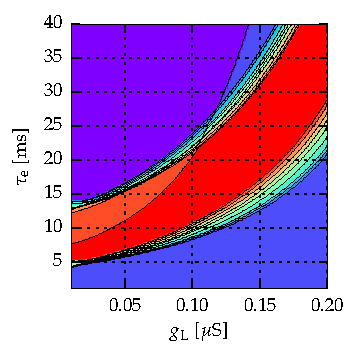
\includegraphics[trim=2mm 2mm 2mm 2mm,clip]{media/chp4/evaluation/i6_ex_sc1_Train_N10_XgL_YtauE_pBin_Train_AdIfCondExp_small.pdf}%
		\label{fig:ns_adex_sts1}
	}%
	\subbottom[AdEx, \STI (II)]{%
		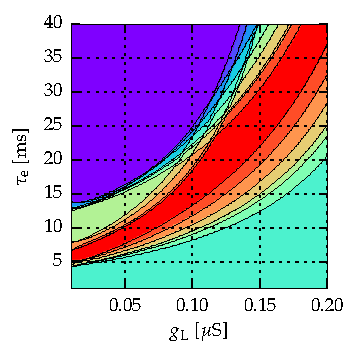
\includegraphics[trim=2mm 2mm 2mm 2mm,clip]{media/chp4/evaluation/i7_ex_sc1_Train_N10_XgL_YtauE_pBin_Train_AdIfCondExp_small.pdf}%
		\label{fig:ns_adex_sts2}
	}
	\subbottom[AdEx, SGMO]{%
		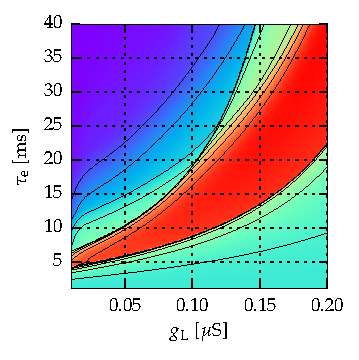
\includegraphics[trim=2mm 2mm 2mm 2mm,clip]{media/chp4/evaluation/i10_ex_sc1_SgMo_XgL_YtauE_pSoft_SgMo_AdIfCondExp_small.pdf}%
		\label{fig:ns_adex_sgmo}
	}%
	\subbottom[AdEx, \STII]{%
		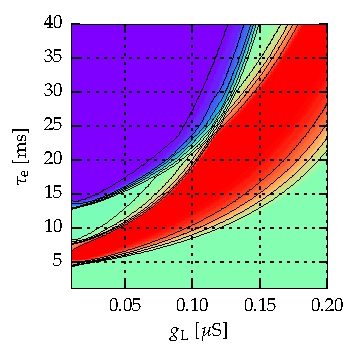
\includegraphics[trim=2mm 2mm 2mm 2mm,clip]{media/chp4/evaluation/i8_ex_sc1_Train_N100_XgL_YtauE_pBin_Train_AdIfCondExp_small.pdf}%
		\label{fig:ns_adex_st}
	}
	\subbottom[LIF, SGMO]{%
		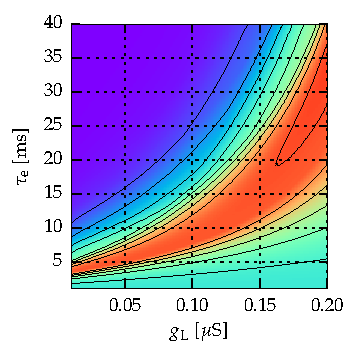
\includegraphics[trim=2mm 2mm 2mm 2mm,clip]{media/chp4/evaluation/i5_ex_sc1_SgMo_XgL_YtauE_pSoft_SgMo_IfCondExp_small.pdf}%
		\label{fig:ns_lif_sgmo}
	}%
	\subbottom[AdEx, SGSO]{%
		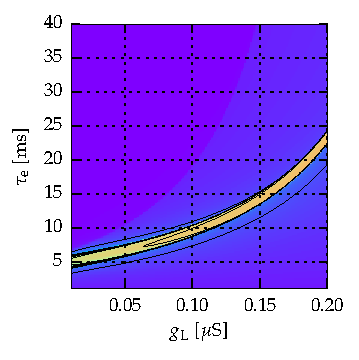
\includegraphics[trim=2mm 2mm 2mm 2mm,clip]{media/chp4/evaluation/i9_ex_sc1_SgSo_XgL_YtauE_pSoft_SgSo_AdIfCondExp_small.pdf}%
		\label{fig:ns_adex_sgso}
	}
	\hspace*{7mm}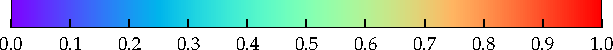
\includegraphics{media/chp4/evaluation/colorbar.pdf}
	\caption[Design space exploration results]{Selected results of the first design space exploration sweep (over \Gl and \TauE). Colour-coded is the evaluation result $\Pgen \in [0, 1]$. The contour lines correspond to the ticks on the colour bar. Only a portion of the design space exploration is shown. Refer to the text for more details.}
	\label{fig:ns}
\end{figure}
\marginnote{An interesting effect that can be found in \cref{app:evaluation_measure_comparison} is noise produced by the \STII measure in conjunction with the \AdEx neuron for large \Gl and small \TauE. This is believed to be caused by the adaptive step size integrator in conjunction with the fast neuron dynamics in this region. The author assures that this kind of noise is not unique to the spike train measure. If desired, it can be eliminated by employing a constant step size integrator at the cost of magnitudes larger runtimes.}
\cref{fig:ns} shows visualisations of the evaluation measures for subregions of the first parameter sweep. \cref{fig:ns_adex_sts1,fig:ns_adex_sts2} show two independent runs of \STI for an \AdEx neuron. The results differ significantly from each other. There are clearly visible discrete steps in the result. Upon first visual inspection, the \SGMO measure in \cref{fig:ns_adex_sgmo} replicates \STII in \cref{fig:ns_adex_sts1}, while featuring a clear gradient leading towards the centre region with high optimality. In contrast, \STII is uniform in vast regions of the design space. The gradient of the \SGMO measure is even clearer in \cref{fig:ns_lif_sgmo}, where the result for the \LIF neuron is shown. Interestingly, the region with maximum optimality is more concentrated than in the results for the \AdEx neuron. The result for the \SGSO measure in \cref{fig:ns_adex_sgso} is visually distinct from the others, yet the location of the region with high optimality is largely the same. The \SGSO measure furthermore shows a subtle gradient. Upon closer inspection it becomes apparent that the maximum regions of the \SGMO and \SGSO measures do not entirely cohere with those of \STII. They seem to extend a little further towards larger $\Gl$. The complete set of results including the second exploration can be found in \cref{app:evaluation_measure_comparison}. Similar to the manually picked examples shown here, all measures exhibit a pronounced region with maximum optimality \Pgen. Unsurprisingly, \SGSO and \SGMO feature a clear gradient, whereas \STII does not.


\paragraph{Discussion}
A plausible explanation of the runtime differences between the individual exploration runs and the \AdEx and \LIF neuron is the adaptive step size integrator. The exponential spike generation mechanism of the \AdEx neuron apparently requires smaller integration steps, causing a higher runtime. The sweep over \ETh is likely to produce many output spikes for small \ETh, which explains the additional slowdown and especially the disproportionate runtime increase for the \SGMO measure: here, the runtime directly depends on the number of output spikes. The differences in runtime should be seen as a strong argument for the adaptive step size integrator, as it is responsible for the major speedups in parameter space regions with few output spikes.

The empirical results of the evaluation measures themselves fit well into the conjectures made in \cref{sec:evaluation_measure_theoretical}. Most interestingly, the \SGMO measure indeed provides a very good approximation of the \STII measure at a fraction of a runtime, as well as a smooth gradient. Compared to the \AdEx neuron, the measures for the \LIF neuron model exhibit more smooth results, which is likely due to the exponential attractor dynamics in the \AdEx neuron. The visually distinct appearance of the \SGSO measure is likely caused by the multiplication of four terms in \cref{eqn:pth,eqn:preset,eqn:psgso}, which, despite the heavy-tailed sigmoids, tends to generate small values. Careful tuning of the underlying distribution meta-parameters may improve the predictive power of both the \SGSO and the \SGMO measure.

\subsection{Automated parameter optimisation}
\label{sec:optimisation}

The \SGMO and \SGSO measures exhibit a smooth gradient in two dimensional parameters sweeps, like those shown above. The gradient could be followed by a simple optimisation algorithm to find the global subspace maximum. It is doubtful, that this property translates to higher-dimensional subspaces, where it is likely that local maxima are omnipresent. Furthermore, the claim, that the gradient supports parameter optimisation has not been tested yet. In the following, we perform a benchmarking experiment which tests the suitability of the single neuron evaluation measures for the task they were designed for -- parameter optimisation.

\paragraph{Methods}
\begin{table}[t]
	\centering
	\small
	\renewcommand{\arraystretch}{1.1}
	\begin{tabular}{rrrrr}
		\toprule
		\multicolumn{5}{c}{\spacedlowsmallcaps{Scenarios for neuron parameter optimisation}} \\
		\midrule
		\multicolumn{5}{c}{\textit{Relevant network parameters}} \\
		\midrule
		&&{\footnotesize\spacedlowsmallcaps{Scenario I}}
		 &{\footnotesize\spacedlowsmallcaps{Scenario II}}
		 &{\footnotesize\spacedlowsmallcaps{Scenario III}} \\

		Ones in the input & $\nOnesIn$ & 3 & 3 & 3 \\
		Population size & $\populationSize$ & 1 & 1 & 3\\

		\midrule
		\multicolumn{5}{c}{\textit{Data encoding parameters}} \\
		\midrule
		&&{\footnotesize\spacedlowsmallcaps{Scenario I}}
		 &{\footnotesize\spacedlowsmallcaps{Scenario II}}
		 &{\footnotesize\spacedlowsmallcaps{Scenario III}} \\

		Input burst size & $\burstSizeIn$ & 1 & 3 & 3 \\
		Output burst size & $\burstSizeOut$ & 1 & 3 & 3 \\
		Interspike interval & $\isi$ & \SI{10}{\milli\second} & \SI{10}{\milli\second} & \SI{10}{\milli\second} \\
		Sample interval & $\timeWindow$ & \SI{200}{\milli\second} & \SI{200}{\milli\second} & \SI{200}{\milli\second} \\

		\midrule
		\multicolumn{5}{c}{\textit{Noise parameters}} \\
		\midrule
		&&{\footnotesize\spacedlowsmallcaps{Scenario I}}
		 &{\footnotesize\spacedlowsmallcaps{Scenario II}}
		 &{\footnotesize\spacedlowsmallcaps{Scenario III}} \\

		Jitter & \jitter & \SI{5}{\milli\second} & \SI{5}{\milli\second} & \SI{5}{\milli\second} \\

		\midrule
		\multicolumn{5}{c}{\textit{Resulting input and output spike counts}} \\
		\midrule
		&&{\footnotesize\spacedlowsmallcaps{Scenario I}}
		 &{\footnotesize\spacedlowsmallcaps{Scenario II}}
		 &{\footnotesize\spacedlowsmallcaps{Scenario III}} \\

		Upper threshold & $\threshOne$ & 3 & 9 & 27\\
		Lower threshold & $\threshZero$ & 2 & 6 & 18\\
		Output spike count & $\nOut$ & 1 & 3 & 3\\
 		\bottomrule
	\end{tabular}
	\caption[Scenarios for neuron parameter optimisation]{Scenarios for the neuron parameter optimisation test. The table shows the chosen system parameters (\cref{tbl:design_space}) and the resulting input and output target spike counts. The noise parameters $\pFp$, $\pFn$, $\jitterOffs$, $\jitterWSyn$ are set to zero since they cannot be tested with the \SGSO and \SGMO measure, or, in the case of \jitterOffs, are not explicitly modelled. System parameters not listed here are irrelevant for single neuron evaluation.}
	\label{tbl:scenarios}
\end{table}
\marginnote{Automated parameter optimisation itself is not the focus of this thesis and surly more advanced experiments and optimisation methods should be employed in future work.}
Goal of the experiment is to optimise the parameters of an \LIF and an \AdEx neuron with respect to the three single neuron evaluation measures, \STII, \SGSO and \SGMO. The system parameters are chosen according to three scenarios presented in \cref{tbl:scenarios}. The first scenario tests single output spikes, the second bursts of $\burstSizeIn = \burstSizeOut = 3$ spikes, and the third a neuron population of $\populationSize = 3$ neurons. For the \LIF neuron, the only potential being optimised is \ETh, for the \AdEx neuron \EThEff. Furthermore, \Cm is kept constant. Starting point of the optimisation are the initial neuron parameters \nParams shown in \cref{tbl:initial_parameters}.

The optimisation method itself is a standard Nelder and Mead minimisation algorithm, a multidimensional generalisation of the bisection method also known as \emph{Downhill Simplex} \cite{nelder1965simplex}. Advantages of the algorithm are its simplicity and implicit gradient calculation. A major disadvantage is its slow convergence \cite{press2007numerical_downhill}. The implementation provided as part of \AdExpSim features concurrent parallel execution of slightly varying vectors and automated restart for the escape from local minima, support for arbitrary parameter constraints and discrete parameters, such as \wsyn in \mbox{\NMPM} and Spikey. Apart from this, the algorithm follows the implementation presented in Numerical Recipes \cite{press2007numerical_downhill}.

\paragraph{Results}
\begin{table}[p]
	\centering
	\small
	\begin{tabular}{l r r r r r r r}
		\toprule
 		\multicolumn{8}{c}{\spacedlowsmallcaps{Initial evaluation measure optimality values}} \\
		\midrule

			\multicolumn{2}{l}{\textit{Scenario}}
			& \multicolumn{3}{c}{\textit{LIF}}
			& \multicolumn{3}{c}{\textit{AdEx}} \\

			\cmidrule(l){3-5}\cmidrule(l){6-8}

			&
			& \spacedlowsmallcaps{ST$_\mathrm{100}$}
			& \spacedlowsmallcaps{SGSO}
			& \spacedlowsmallcaps{SGMO}
			& \spacedlowsmallcaps{ST$_\mathrm{100}$}
			& \spacedlowsmallcaps{SGSO}
			& \spacedlowsmallcaps{SGMO} \\

			\cmidrule(r){1-2}\cmidrule(l){3-3}\cmidrule(l){4-4}\cmidrule(l){5-5}\cmidrule(l){6-6}\cmidrule(l){7-7}\cmidrule(l){8-8}

			\multirow{3}{*}{Initial}
				& \spacedlowsmallcaps{I}
					& 0.78 & 0.43 & 0.89
					& 0.46 & 0.11 & 0.51\\
				& \spacedlowsmallcaps{II}
					& 0.28 & / & 0.22
					& 0.00 & / & 0.16\\
				& \spacedlowsmallcaps{III}
					& 0.00 & / & 0.00
					& 0.00 & / & 0.00\\

		\midrule
		\multicolumn{8}{c}{\spacedlowsmallcaps{Final evaluation measure optimality values}} \\
		\midrule

			  \multirow{2}{2cm}{\vspace{2mm}\textit{\mbox{Target measure/} Scenario}}
			&& \multicolumn{3}{c}{\textit{LIF}}
			& \multicolumn{3}{c}{\textit{AdEx}} \\

			\cmidrule(l){3-5}\cmidrule(l){6-8}

			&
			& \spacedlowsmallcaps{ST$_\mathrm{100}$}
			& \spacedlowsmallcaps{SGSO}
			& \spacedlowsmallcaps{SGMO}
			& \spacedlowsmallcaps{ST$_\mathrm{100}$}
			& \spacedlowsmallcaps{SGSO}
			& \spacedlowsmallcaps{SGMO} \\

			\cmidrule(r){1-2}\cmidrule(l){3-3}\cmidrule(l){4-4}\cmidrule(l){5-5}\cmidrule(l){6-6}\cmidrule(l){7-7}\cmidrule(l){8-8}

			\multirow{3}{*}{\STII}
				& \spacedlowsmallcaps{I}
					& $\diamond$ \textbf{1.00} & 0.40 & 0.76
					& \textbf{1.00} & 0.01 & 0.09 \\
				& \spacedlowsmallcaps{II}
					& \textbf{0.52} & / & 0.00
					& \textbf{0.46} & / & 0.00 \\
				& \spacedlowsmallcaps{III}
					& \textbf{0.00} & / & 0.00
					& \textbf{0.39} & / & 0.00 \\

			\cmidrule(r){1-2}\cmidrule(l){3-3}\cmidrule(l){4-4}\cmidrule(l){5-5}\cmidrule(l){6-6}\cmidrule(l){7-7}\cmidrule(l){8-8}

			\SGSO
				& \spacedlowsmallcaps{I}
					& 1.00 & $\diamond$ \textbf{0.61} & 0.00
					& 0.92 & \textbf{0.70} & 0.91 \\

			\cmidrule(r){1-2}\cmidrule(l){3-3}\cmidrule(l){4-4}\cmidrule(l){5-5}\cmidrule(l){6-6}\cmidrule(l){7-7}\cmidrule(l){8-8}

			\multirow{3}{*}{\SGMO}
				& \spacedlowsmallcaps{I}
					& 0.73 & 0.33 & $\diamond$ \textbf{0.98}
					& 0.56 & 0.50 & \textbf{0.92} \\
				& \spacedlowsmallcaps{II}
					& 0.42 & / & \textbf{0.94}
					& 0.00 & / & \textbf{0.19} \\
				& \spacedlowsmallcaps{III}
					& 0.44 & / & \textbf{0.97}
					& 0.00 & / & \textbf{0.00} \\
			\bottomrule
	\end{tabular}
	\caption[Results of the neuron parameter optimisation experiment]{Initial and final neuron evaluation measure optimality values. The top part of the table shows the initial evaluation measure optimality values \Pgen prior to optimisation, with respect to the three system parameter scenarios (rows). The bottom part of the table shows the same evaluation measures after the parameters have been optimised with respect to a scenario and target optimisation measure (rows). Bold values correspond to the final values of the target measure. $\diamond$ The final neuron parameter vectors for these results are shown in \cref{tbl:optimisation_experiment_values}.}
	\label{tbl:optimisation_experiment_results}
\end{table}
\begin{table}[p]
	\centering
	\small
	\centering
	\small
	\renewcommand{\arraystretch}{1.2}
	\begin{tabular}{c r r r r r r r}
		\toprule
		\multicolumn{8}{c}{\spacedlowsmallcaps{Optimised LIF neuron parameters}} \\
		\midrule

		&  & &
			& \spacedlowsmallcaps{Init.}
			& \spacedlowsmallcaps{ST$_\mathrm{100}$}
			& \spacedlowsmallcaps{SGSO}
			& \spacedlowsmallcaps{SGMO} \\

		& Membrane cap. & \Cm & {[\si{\nano\farad}]}
			& 1.00 & 1.00 & 1.00 & 1.00\\
		$\circ$ & Leak conductance & \Gl & {[\si{\nano\siemens}]}
			& 50.00 & 45.50 & 13.40 & 14.50\\
		& Leak potential & \El & {[\si{\milli\volt}]}
			& -70.00 & -70.00 & -70.00 & -70.00 \\
		$\circ$  & Threshold potential & \ETh & {[\si{\milli\volt}]}
			& -54.00 & -52.50 & -48.23 & -65.80 \\
		& Reset potential & \Ereset & {[\si{\milli\volt}]}
			& -80.00 & -80.00 & -80.00 & -80.00 \\
		$\circ$ & Refractory period & \TauRef & {[\si{\milli\second}]}
			& 0.00 & 0.00 & 0.00 & 0.00 \\
		& Synapse potential & \Ee & {[\si{\milli\volt}]}
			& 0.00 & 0.00 & 0.00 & 0.00 \\
		$\circ$ & Synapse time & \TauE & {[\si{\milli\second}]}
			& 5.00 & 5.37 & 0.10 & 1.20 \\
		$\circ$ & Synapse weight & \wsyn & {[\si{\nano\siemens}]}
			& 30.00 & 36.25 & 1477 & 19.23 \\
		\bottomrule
	\end{tabular}
	\caption[Optimised LIF neuron parameters]{Initial and optimised \LIF neuron parameters. The corresponding optimality values \Pgen are shown in \cref{tbl:optimisation_experiment_results}, where they are marked with a \enquote{$\diamond$}-symbol. $\circ$ These parameter dimensions were optimised.}
	\label{tbl:optimisation_experiment_values}
\end{table}
A striking property of the results shown in \cref{tbl:optimisation_experiment_results} is incoherence of the evaluation measure optimality values. Optimising with \STII as target measure results in optimality values below those for unoptimised parameters for the \SGMO and \SGSO measures. Optimisation with \SGSO results in zero optimality according to the \SGMO measure for the \LIF neuron. Yet, parameter vectors optimised with \SGSO receive a high lateral score from the \STII measure. Optimisation for \SGMO results in mediocre values for both \STII and \SGSO. Still at least for \emph{Scenario I}, optimisation significantly increases the optimality value of the current target measure (bold values in the table). Remarkably, the \SGMO measure is capable of finding \enquote{optimal} solutions for the second and third scenario in conjunction with a \LIF neuron, starting from a small optimality values.

\cref{tbl:optimisation_experiment_values} shows the optimised \LIF neuron parameters for the first system parameter scenario. The chosen parameters differ significantly between the target measures. The \SGSO measure converges towards a rather peculiar parameter combination, with a very small synapse time constant \TauE, small leak conductance \Gl, and a relatively large synapse weight. Yet, despite their differences, this parameter vector and the parameter vector optimised by \STII, are evaluated with maximum optimality by \STII.

\paragraph{Discussion}
The incoherence of the optimality values is most likely influenced by three factors: deficiencies of the evaluation measures, a lack of regularisation, and different semantics of the values. Problems with the evaluation measures have already been observed in the previous experiments, where \SGSO and \SGMO do not entirely overlap with \STII. The lack of parameter regularisation allows grotesque parameter combinations, as those found for the \LIF neuron and \emph{Scenario I}, which in return are likely to be rejected by other evaluation measures. The semantics of the \STII measure are entirely different from \SGSO and \SGMO. A non-spiking neuron will always produce a value of $\PST = 0.5$, as half of all spike groups are successful. Such a behaviour would be scored with a near zero value by \SGSO and \SGMO. On the other hand, the spike train measure is extremely harsh, as any deviation in the output spike count of just a single spike out of multiple is counted as failure.

\marginnote{The \STII measure only works as well as presented, because the optimiser probabilistically reinitialises the parameter vectors once they converge, which causes the optimiser to eventually \enquote{jump} over the discrete steps in \STII.}
Despite these issues, the results clearly show that parameter optimisation is indeed feasible with the presented methods. All measures find optimal (with respect to themselves) parameter combinations for \emph{Scenario I}. The fact that optimisation with \SGMO finds such parameters for the \LIF neuron in the intrinsically difficult scenarios \emph{II} and \emph{III} hints at the power of smooth gradients in the parameter space in conjunction with the chosen optimisation method. Nevertheless, further improvement of \SGMO is inevitable, since the parameters will not fulfil the \BiNAM requirements in practice ($\PST < 0.5$). As long as the neuron should only produce a single output spike, the \SGSO measure seems to be a viable option for parameter selection.

\section{Conclusion}
In this chapter we described the design space, and presented and compared three approaches to single neuron evaluation. A comprehensive software framework has been developed for the simulation and evaluation of single neurons. Two-dimensional parameter sweeps over parts of the design space show a rather well-behaved landscape with pronounced, coherent regions with high optimality. Nevertheless, the parameter optimisation experiment demonstrates the perils of high-dimensional parameter spaces. Although the \SGMO measure does not perform as well as anticipated, it and its underlying fractional spike count measure seem to be viable approaches to neuron parameter optimisation.

Until now, the predictive power of the single neuron evaluation measures have not been examined regarding the ground truth, namely full network simulation. This examination is one of the goals of the next \cref{chp:experiments}, in which we finally execute the \BiNAM on actual neuromorphic hardware and -- amongst others -- compare the full network evaluation results with the predictions from the single neuron evaluation.
